\documentclass{svmult}

\usepackage[utf8]{inputenc}
\usepackage[table]{xcolor}
\usepackage{url}
\usepackage{hyperref}

\usepackage[numbers]{natbib}
%\usepackage[switch]{lineno}

\usepackage{amsmath} % assumes amsmath package installed
\usepackage{amssymb}  % assumes amsmath package installed

\usepackage{enumerate}
\usepackage{paralist} %for inline lists

\usepackage{array}
\usepackage{amsmath}

\usepackage{subfigure}

\usepackage{pseudocode}
\usepackage{alltt}

%diagrams
\usepackage{tikz}
\usetikzlibrary{shapes,trees}

\usepackage{lscape}

\usepackage{fixme}
\fxusetheme{color}

%%%%%%%%%%%% Custom macros %%%%%%%%%%%%%

%Name of the speaker in a chat
\newcommand{\chatN}[1]{{\footnotesize \textsf{#1}}}
\newcommand{\concept}[1]{{\footnotesize \texttt{#1}}}

\newcommand{\stmt}[1]{{\footnotesize $\langle$\stmttt#1\relax$\rangle$}}
\newcommand{\rawstmt}[1]{{\footnotesize \stmttt#1\relax}}
\def\stmttt#1 #2 #3\relax{{\tt#1} {\bf{\tt #2}} {\tt #3}}

\newcommand{\setstmt}[1]{{\footnotesize [\setstmttt#1\relax]}}
\def\setstmttt#1,#2\relax{\rawstmt{#1}, \rawstmt{#2}}

\usepackage{xspace}
\newcommand{\ie}{i.e.\xspace}
\newcommand{\cf}{cf\xspace}
\newcommand{\eg}{e.g.\xspace}

%------------------------------------------------------------------------- 

\begin{document}
%\linenumbers

% Alternate row background in tables
\rowcolors{2}{gray!10}{white}

\title*{Towards Grounding Human-Robot Interaction}

\author{
Séverin Lemaignan,
Rachid Alami,
Amit Kumar Pandey,
Matthieu Warnier,
Julien Guitton
}
\authorrunning{Séverin Lemaignan et al.}

\institute{ 
	Séverin Lemaignan \and Rachid Alami \and Amit Kumar Pandey \and Matthieu Warnier \and Julien Guitton
	\at
	CNRS - LAAS, 7 avenue du Colonel Roche, F-31077 Toulouse, France\\
	Université de Toulouse, UPS, INSA, INP, ISAE, LAAS, F-31077 Toulouse, France\\
    \email{severin.lemaignan@plymouth.ac.uk, rachid.alami@laas.fr}
}

\maketitle

%\clearpage
%\setcounter{minitocdepth}{2}
%\dominitoc
%\clearpage

\begin{abstract}\newline

Effective human-robot interaction requires to establish common grounds between
the robot and the human user: the robot needs to perceive and represent what
the human knows, what she or he can do and ultimately want to do. It must then
accordingly come up with appropriate behaviours.

This complex challenge lays at the heart of a lot of academic research in
human-robot interaction (HRI). We present in this chapter our current
understanding of the problem, from the perspective of symbolic cognition: our
robots build in real-time complex symbolic models of the environment and the
surrounding humans, and use these grounded models to achieve advanced cognitive
behaviours like collaborative task planning or dialogue understanding.

We have attempted to present our approach in a constructive way: all the
presented techniques are matched with open-source software implementations, and
we besides provide are rich set of pointers to the literature. This should
hopefully enable the interested reader to quickly form a useful picture of the
field.

\end{abstract}



%%%%%%%%%%%%%%%%%%%%%%%%%%%%%%%%%%%%%%%%%%%%%%%%%%%%%%%%%%%%%%%%%%%%%%%%%%%%
%%%%%%%%%%%%%%%%%%%%%%%%%%%%%%%%%%%%%%%%%%%%%%%%%%%%%%%%%%%%%%%%%%%%%%%%%%%%
\section{Introduction}

\subsection{Grounding the Human Interaction: the Challenges}

{\em Aperitif time. Sitting down in his comfortable armchair, Tom gives a look
at the empty table. ``{\em Hey robot, put two glasses and this bottle on the
tray!}'' ``{\em And bring that over there.}''. The robot asks ``{\em The
Martini or the Porto?}'' ``{\em Bring both!}'' answers Tom. The robot prepares
the order and smoothly brings the tray to the table.} (Fig.~\ref{fig|vpt}).

\begin{figure}%[!ht] 
	\centering
	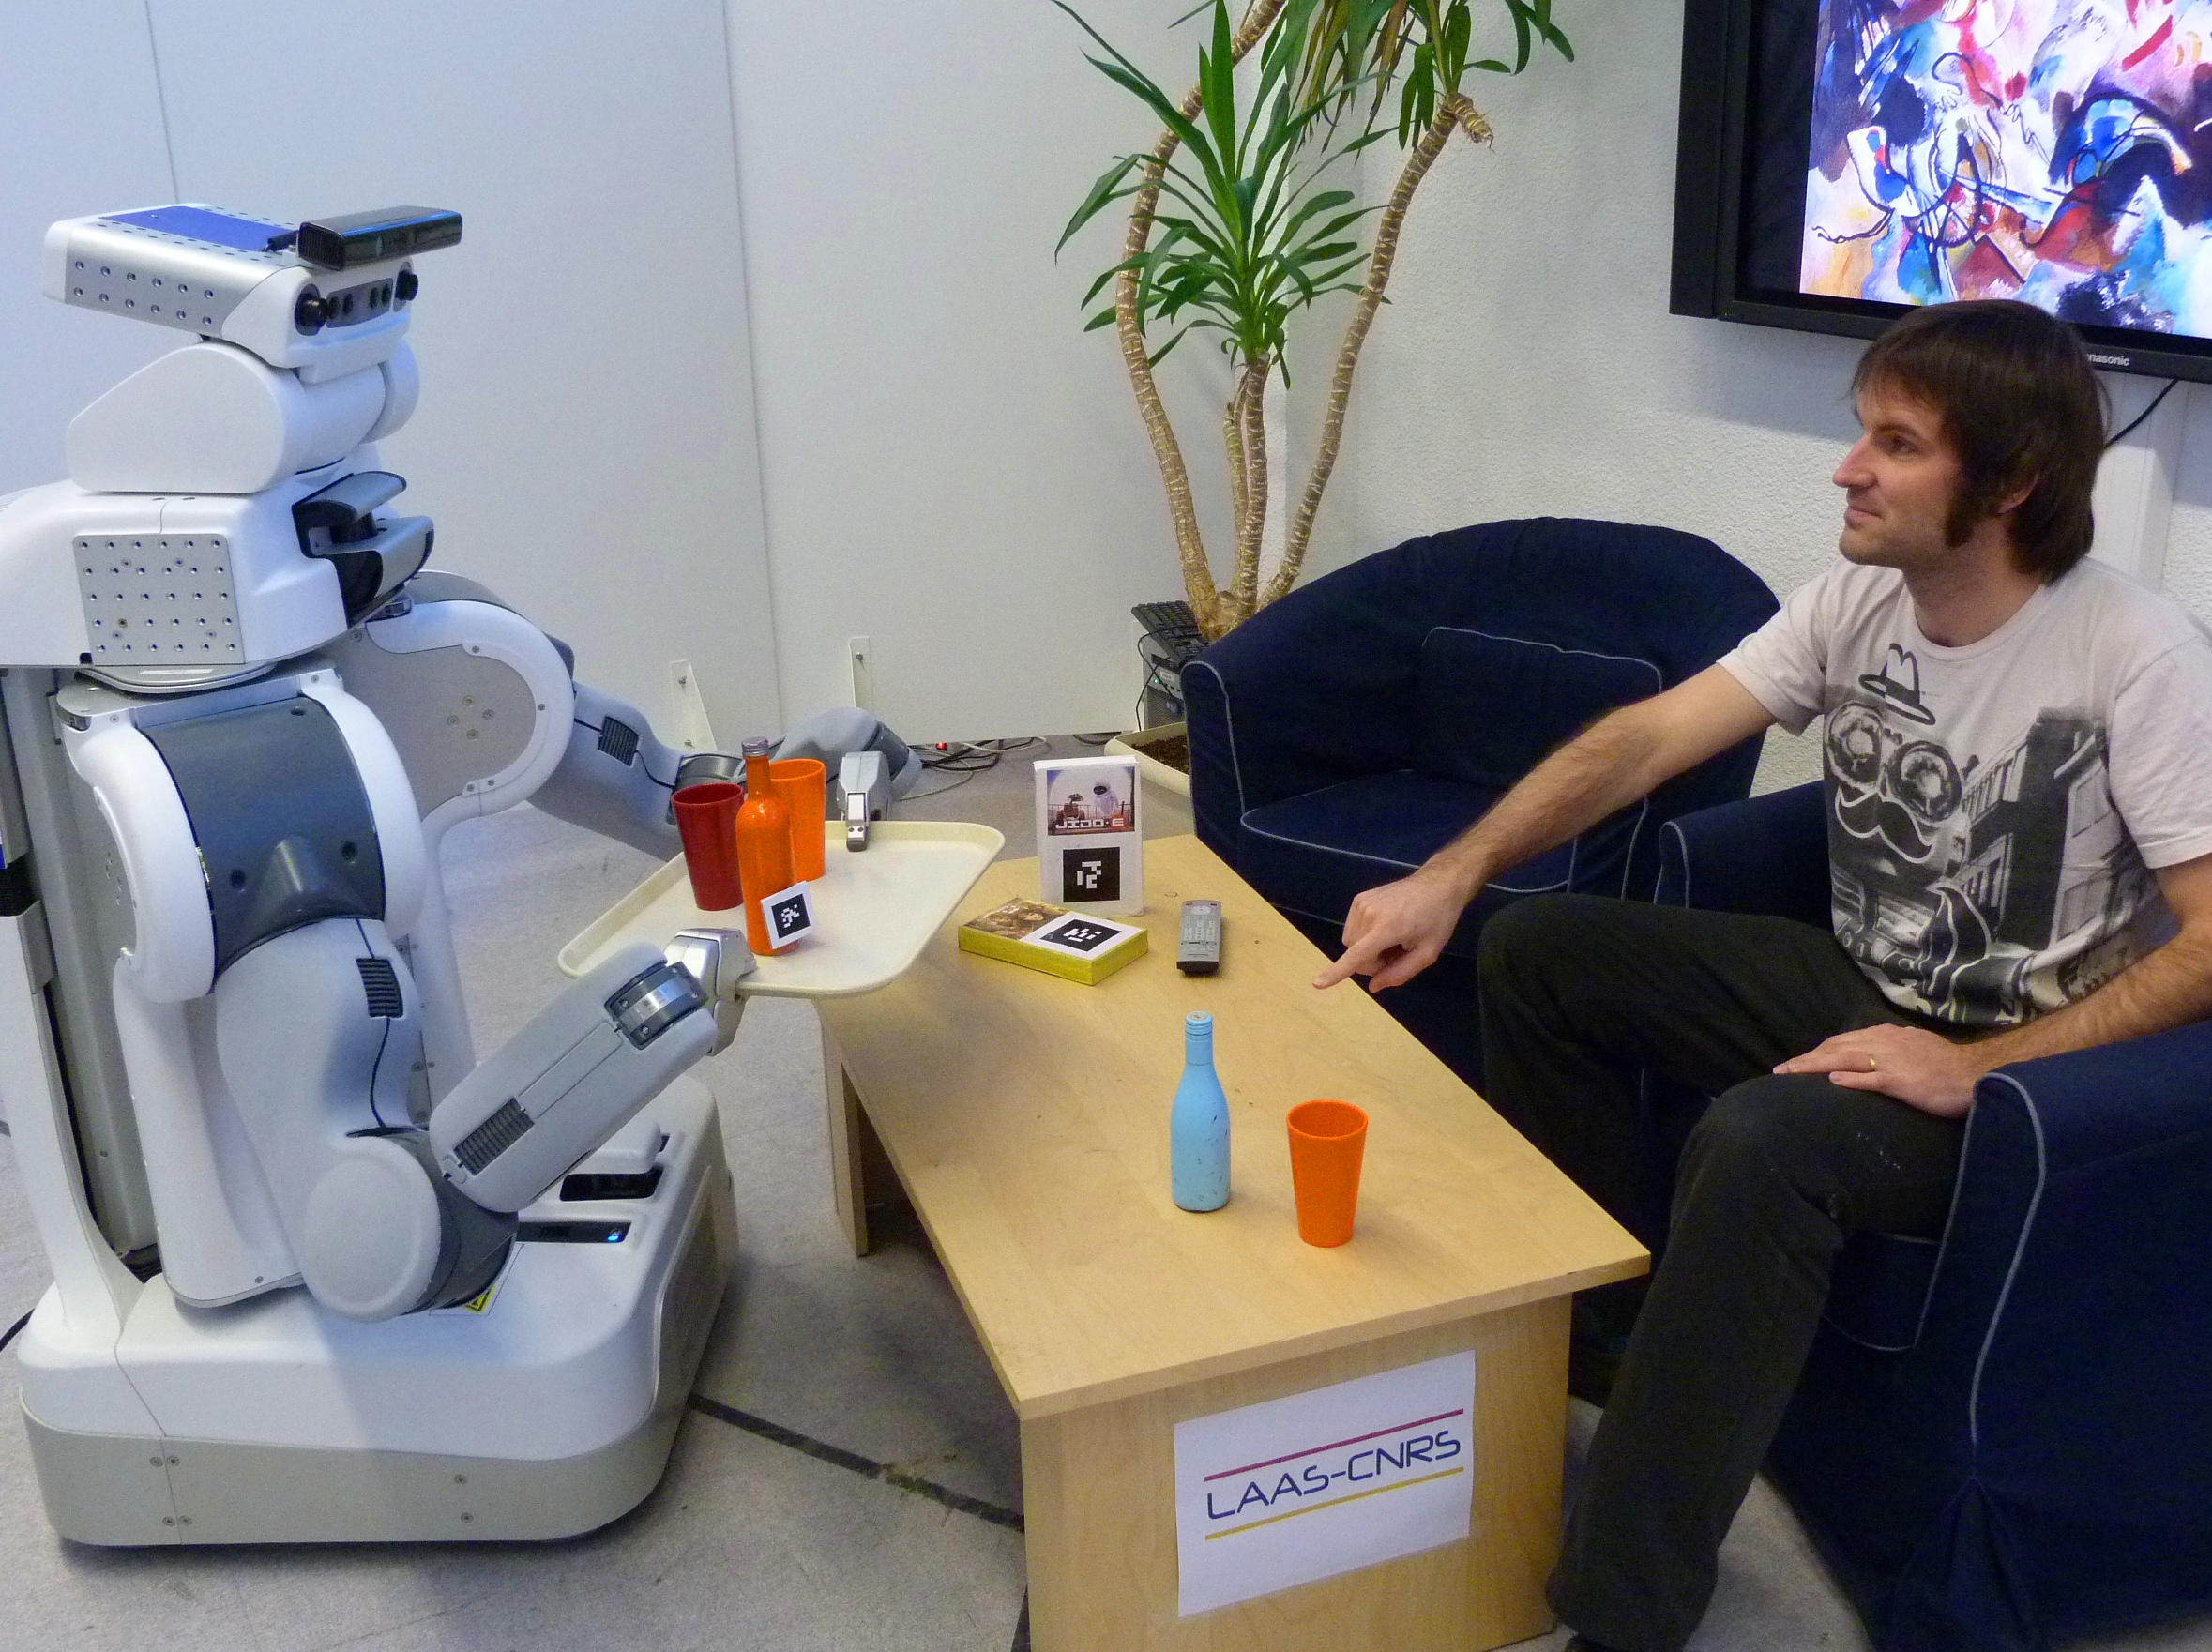
\includegraphics[width=0.8\linewidth]{figs/aperitif_time.jpg} 

	\caption{Interacting with the robot in an everyday situation: the human
	asks for help in vague terms, the robot takes into account the human's {\it
	a priori} knowledge and spatial perspective to refine its understanding of
	the question.} 

	\label{fig|vpt} 
\end{figure}

This is an example of the kind of natural interaction that is a short-term
target for the human-robot interaction community.

This simple scenario belongs to the broad class of \emph{interactive
manipulation problems}: several agents agree a (more or less implicit) joint
goal that requires some sort of cooperation to be successfully achieved. These
problems involve both dialogue and manipulation and are often iterative.


\begin{figure}[htb]
\centering
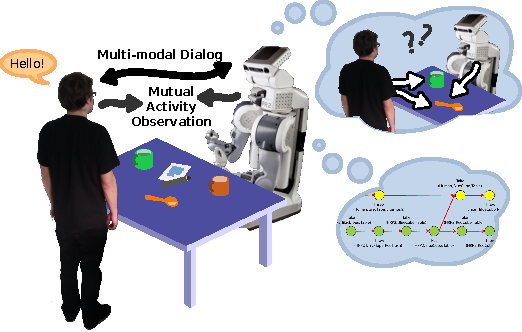
\includegraphics[width=9cm]{figs/grounding_robot.pdf}
\caption{Robot reasoning about HRI and anticipation of human activities:
  sources of information are multi-modal dialogue and observation of
  the environment and the human activities}
\label{fig|hri-dec}
\end{figure}

Figure~\ref{fig|hri-dec} illustrates some of the aspects of the interaction.
On the side of the robot, several cognitive skills are involved: dialogue
processing through verbal and deictic modalities (what does the human say? what
attitude -- gazes, postures, gestures... -- does he express?), acquisition
and maintainance of one or several models of the environment, not only from the
robot point of view, but also from the other agents' points of view,
anticipation (what are the intentions of the human? Can I predict and
anticipate his/her actions?), planning and control (how would I proceed further
towards the goal?), monitoring of the other agents' activities (do we have an
effective cooperation?) and the overall progress of the task. 

What are the prerequisites for a sentence like ``Robot, put two glasses and
this bottle on the tray'' to be understood by the robot, correctly
interpreted in the spatial context of the interaction, and eventually
transformed into a set of actions? We summarize these challenges in four
categories:

\begin{enumerate}

	\item how to build and maintain a consistent geometric model of the current
	situation, acquired through perception or deduction from previous
	perceptions,

	\item how to build an unambiguous symbolic representation of concepts
	(objects, agents, actions...) underlying the interaction, and practical for
	decision-making processes,

	\item how to establish the joint goal(s), how to build and maintain
	iteratively shared (human-robot) plans, 

	\item how to refine and execute the computed plans, and how to monitor
	those achieved by its human partner?

\end{enumerate}


This chapter focuses on points {\it 1} and {\it 2}. It presents techniques,
developed and used on several real robots, for the creation of a set of
environment models suitable for grounded situation interpretation,
decision-making and control.

The two other items are however important to actually perform the interaction.
Thus we briefly overview a global architecture of a robot able to cooperate
with humans before really focusing on the grounding issues.

%%%%%%%%%%%%%%%%%%%%%%%%%%%%%%%%%%%

\subsection{An Architecture for Interactive Robotics}
 
\begin{figure*}[thpb]
  \centering
  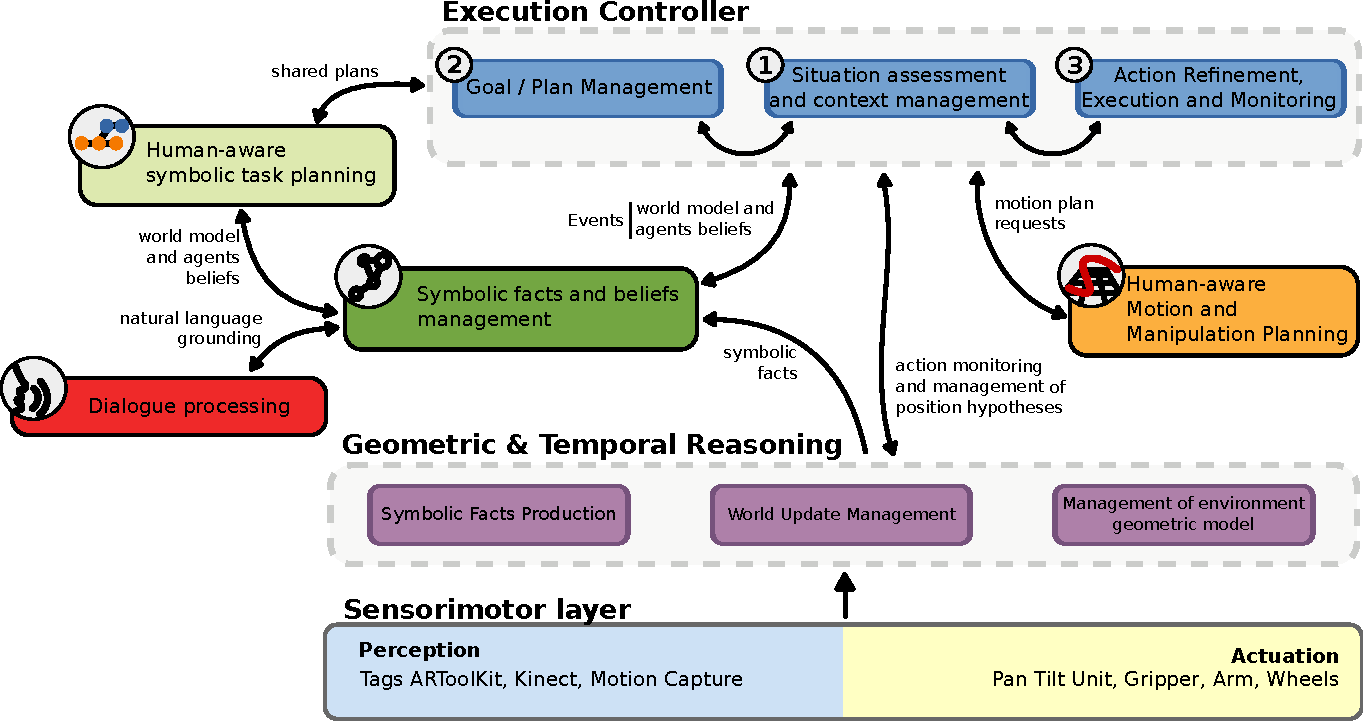
\includegraphics[width=1.0\textwidth]{./figs/architecture-overview.pdf} \\
  \caption {Software architecture for a service robot interacting with humans.}
  \label{fig|archi}
\end{figure*}

Figure~\ref{fig|archi} presents the decisional layer of a service robot as
developed at LAAS~\cite{Alami2011}. The sensorimotor layer (bottom) is
abstracted in an intermediate 3D model where geometric (and some temporal)
reasoning take place~\cite{Sisbot2011}.

The outcome of the geometric analysis, as well as the result of the dialogue
processing module~\cite{Lemaignan2011a}, are stored in a central knowledge
base~\cite{Lemaignan2010}. The symbolic knowledge base triggers events that are
captured by the top-level execution controller.

The controller can rely on two specialized planners: the geometric motion and
manipulation planner~\cite{Sisbot2008, Mainprice2011, Pandey2010} and the
symbolic task planner~\cite{Alili2008}.

The dialogue processing module, as well as the symbolic task planner, also
use the knowledge base to answer questions or initialize the planning domain.

During a typical interaction experiment, the execution controller decides upon a
plan to execute, requires a plan from the task planner, allocates the actions to
the human and the robot, communicates the shared plan, and controls and
monitors its execution. The operation continues until the goal is achieved, is
declared unachievable or is abandoned by the human.


%%%%%%%%%%%%%%%%%%%%%%%%%%%%%%%%%%%
%% Notice on our main assumption %%
%%%%%%%%%%%%%%%%%%%%%%%%%%%%%%%%%%%

\subsubsection*{On object identification and localization}

This architecture makes one important assumption (hidden in the
\emph{Sensorimotor layer} box in Fig.~\ref{fig|archi}): world entities are
assumed to be correctly \emph{perceived}, \emph{localized}, \emph{resolved} and
\emph{uniquely identified} in a robust way.

This means that we assume all relevant entities (\ie the objects the robot has
to interact with) to be actually perceived by the robot when they enter its
field of view, that the perception enables a \emph{good enough} 6D
localization, that the objects are properly resolved (\eg two bottles next to
each other are perceived as two different bottles), and most importantly, that
the objects are robustly identified: each time the exact same object is seen
(possibly under a different angle), it is always labelled with the same,
unique, identifier (the identifier by itself may be completely random, and can
be known at runtime only).

This assumption translates during experiments into technical solutions based on
objects tagging with barcode-like labels (for example, some ARToolkit tags can
be seen on Fig.~\ref{fig|vpt}) that allows the robot to localize and identify
these objects.

Numerous work, some of them presented earlier in this book, focus on dealing
with resolution and identification issues.  We will not further discuss them
here.

%%%%%%%%%%%%%%%%%%%%%%%%%%%%%%%%%%%


\subsection{Chapter overview}

This chapter walks through the on-line building and use of geometric and
symbolic models of the environment and interacting agents. As far as possible,
we try to present the exact list of symbolic statements issued by the
whole system at runtime.

We first examine how the environment is modelled, from the perspectives of
the robot and the other interacting agents. To this end, we introduce
\emph{Perspective Taking}~\cite{Flavell1992,Tversky1999} and some elements of
\emph{Theory of Mind}~\cite{Scassellati2002}\fxwarning{Check this reference is
relevant here} techniques to efficiently compute perspective-aware models of
the world. 

\emph{Search} and \emph{exploration} policies are also presented, along with
symbolic ways to deal with ill-defined locations.

The next section focuses on the modeling of agents and agents capabilities,
including a geometric approach for the analysis of the potential of actions (we
call them \emph{mightabilities}) of each agent.

Section~\ref{cognitivekernel} presents the central knowledge base that
stores, reasons about, and asynchronously (event-driven) exposes the symbolic
facts to the decision-making components. We also discuss here the role of {\it
a priori} knowledge (also called \emph{common-sense} knowledge).

The following two sections~\ref{sec|hatp} and~\ref{dialogs} present actual
applications of this approach. First, we show how the robot may use the
symbolic models for shared task planning: each agent's model of the world is
used to produce one stream of actions per agent, with synchronization points
between them. Then, we present how multi-modal (verbal and deictic) dialogue
processing is made easier by relying on physically grounded and consistent
symbolic models, using semantics close to human natural language.

Bibliographical notes have been added at the end of each relevant section.  We
also present before the conclusion of the chapter other architectures dedicated
to the grounding of human-robot interaction, along with some references
regarding the specifics of the human-robot interactions.


%%%%%%%%%%%%%%%%%%%%%%%%%%%%%%%%%%%%%%%%%%%%%%%%%%%%%%%%%%%%%%%%%%%%%%%%%%%%
%%%%%%%%%%%%%%%%%%%%%%%%%%%%%%%%%%%%%%%%%%%%%%%%%%%%%%%%%%%%%%%%%%%%%%%%%%%%

\section{Building an Agent-Aware Symbolic Model of the Environment}
\label{sec:situ}

Anchoring perceptions in a symbolic model requires perception abilities and
their symbolic interpretation. In this section we present SPARK (\emph{SPAtial
Reasoning \& Knowledge}~\cite{Sisbot2011}), a situation assessment reasoner
that generates relevant symbolic information from the geometry of the
environment with respect to relations between objects, robots and humans.

\begin{figure}[ht!]
   \begin{center}
%
       \subfigure{
           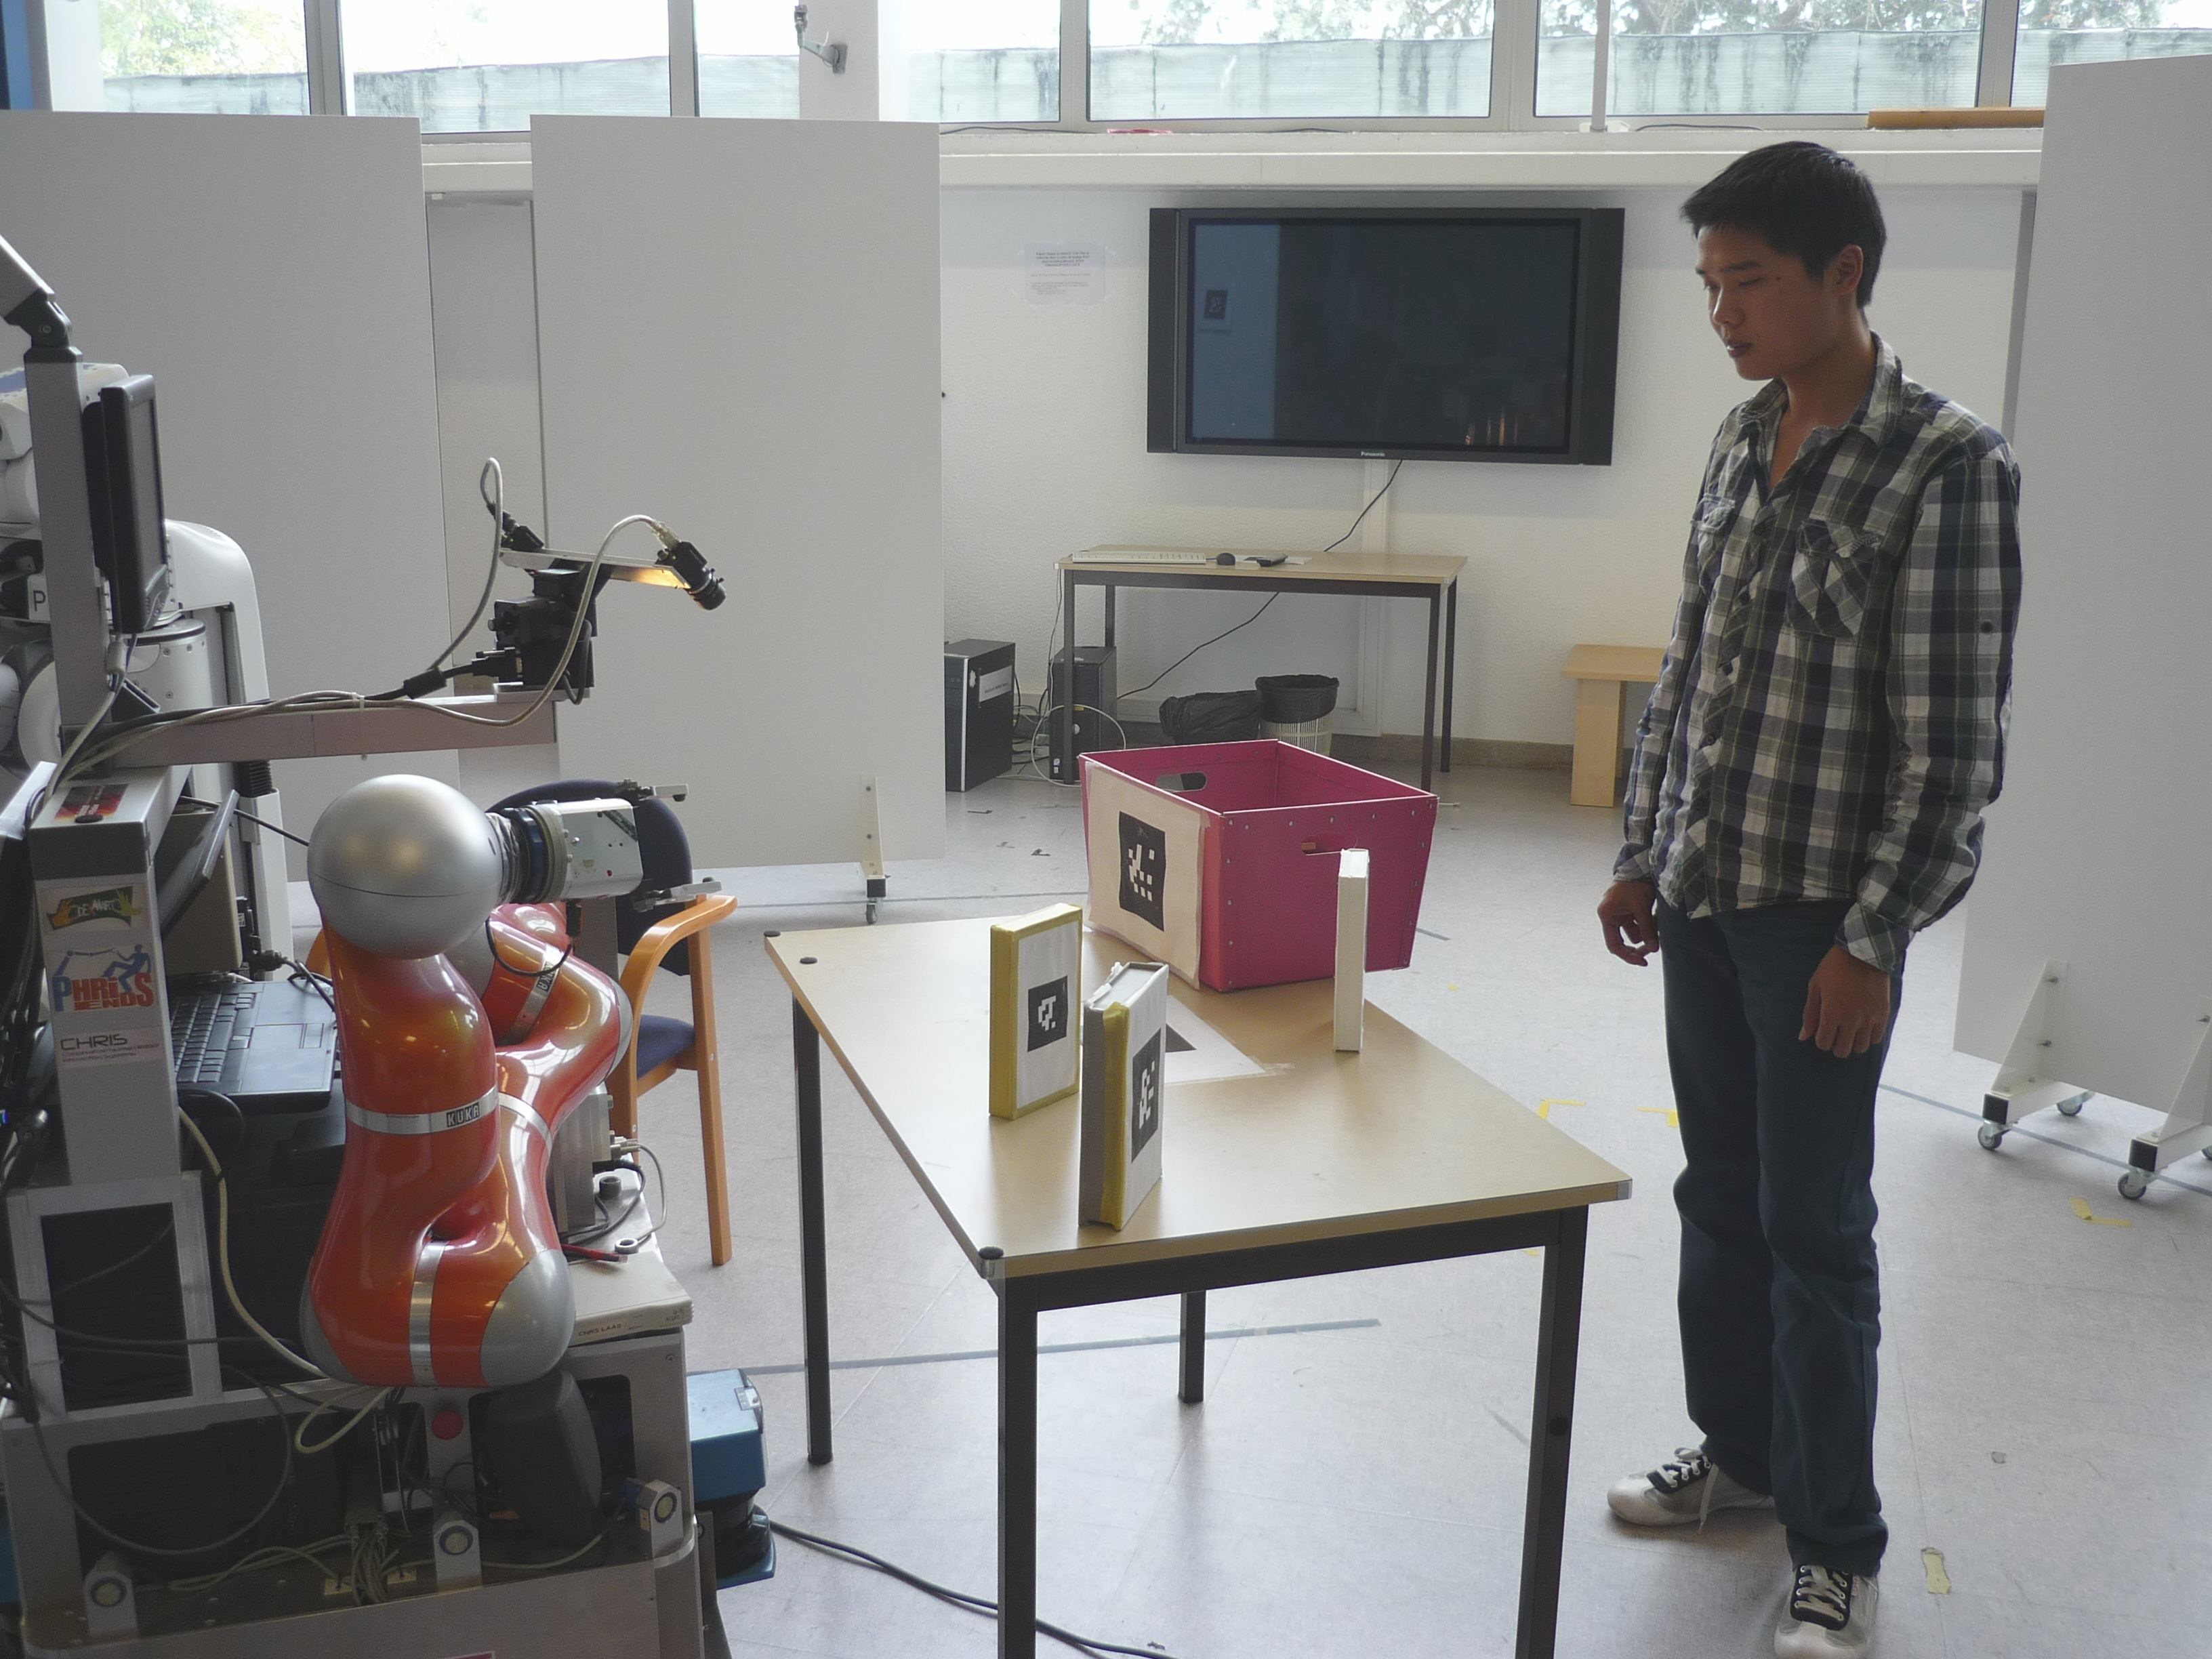
\includegraphics[width=0.5\textwidth]{./figs/etat2-P1010769_brightened-v2.jpg}
       }%
       \subfigure{%
          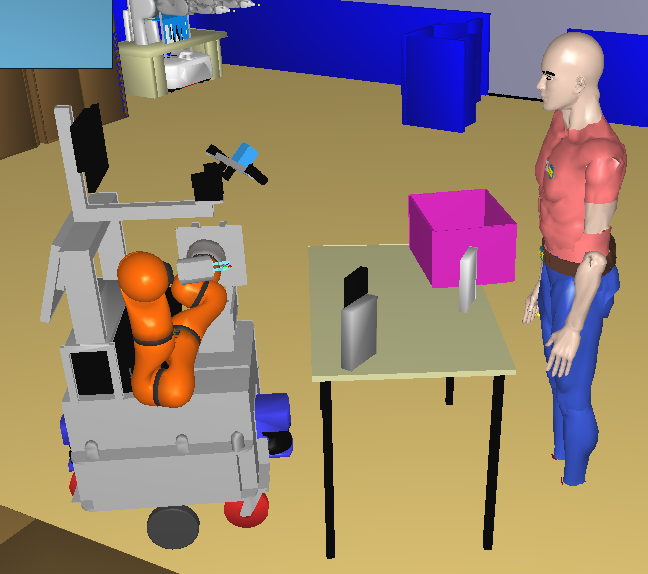
\includegraphics[width=0.43\textwidth]{./figs/etat2_photo.png}
       }\\ %  ------- End of the first row ----------------------%
%
   \end{center}

   \caption{The robot represents at runtime its environment in a 3D model
   resulting of the sensors' inputs fusion (Kinect, motion capture, 2D barcodes
   tracking).}

   \label{fig|spark}

\end{figure}

Figure~\ref{fig|spark} shows a screenshot of the SPARK environment side-by-side
with the real environment: as mentioned in the introduction, objects are
identified and localized through 2D barcodes. The human pose is tracked with
a Microsoft Kinect device (assisted by motion capture to accurately track the
head motion, which is required to compute what the human is looking at).

This geometric model is continuously updated at runtime by the robot.

\subsection{Symbolic locations}

Human commonly refer to the positions of objects with symbolic descriptors
(like \emph{on}, \emph{next to}...) instead of precise, numeric position. These
type of descriptors have been studied in the context of language grounding
(\cite{O'Keefe1999,Matuszek2010,Regier2001,Kelleher2006,Blisard2005}). In this
work we focus on agent-independent symbolic locations (allocentric
representation)  and agent-dependent, relative locations (egocentric
representation).

\subsubsection{Allocentric locations}

We can refer to object locations with respect to other objects in the
environment, such as \emph{above, next to, in}, etc. In this work we compute
three main relations based on the bounding box and center of mass of the
objects (Fig.~\ref{fig|sprelations}): 

\begin{itemize}
	\item \concept{isOn}: computes if an object $O_1$ is on another object $O_2$ by
	evaluating the center of mass of $O_1$ according to the bounding box of $O_2$.

	\item \concept{isIn}: evaluates if an object $O_1$ is inside another object
	$O_2$ based on their bounding boxes $BB_{O_1}$ and $BB_{O_2}$.

	\item \concept{isNextTo}: indicates whether an object $O_1$ is next to another
	object $O_2$. We cannot use a simple distance threshold to determine if two
	objects are next to each other since the relation is highly dependent on the
	dimensions of the objects. For instance, the maximum distance between large
	objects (\eg two houses) to consider them as being next to each other is much
	larger than the maximum distance we would consider for two small objects (\eg
	two bottles). Thus, the relation between the dimensions and the distances of
	the objects are taken into account.  

\begin{figure} 
	\centering
	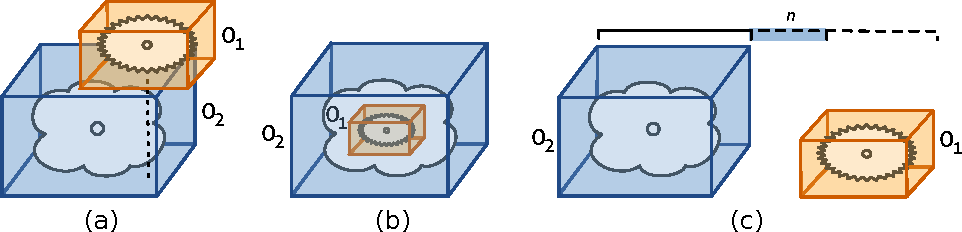
\includegraphics[width=0.95\columnwidth]{figs/spatial_relation.pdf}
	\caption{Spatial relations between two objects: (a) \concept{isOn} relation, 
	(b) \concept{isIn} relation, and (c) \concept{isNextTo} relation.} 
	\label{fig|sprelations} 
\end{figure}

\end{itemize} 

To ensure the different agent models are up-to-date, all these properties are
always computed on-line, each time the current state of the world changes.

Table~\ref{facts|sprelations} lists all the symbolic relationships that are
currently computed by the system.

\begin{table}[h]
    \centering
    \begin{tabular}{p{1.5cm}p{5cm}p{2cm}p{2.7cm}}
	\rowcolor{white}
    \textbf{Subject} & \textbf{Predicate} & \textbf{Object} & \emph{Notes} \\ 
    \hline
	 \concept{Location} & \concept{isAt} $\equiv$ \concept{cyc:objectFoundInLocation}  &  \concept{Location} & \\ 
	 &  $\rightarrow$ \concept{isOn} $\equiv$ \concept{cyc:above\_Touching}  &  & \\ 
	 &  $\rightarrow$ \concept{isIn}  &  & \\ 
	 &  $\rightarrow$ \concept{isNextTo}  & &  \\ 
	 \concept{Location}  & \concept{isAbove} $\equiv$ \concept{cyc:above-Generally}  &  \concept{Location}  &  inverse of \concept{isBelow} \par \concept{isOn} $\Rightarrow$ \concept{isAbove}\\ 
	 \concept{Location}  & \concept{isBelow}  & \concept{Location}  &  inverse of \concept{isAbove}
	\end{tabular}

	\caption{List of statements describing spatial relationships between
	objects. ``$\rightarrow$'' indicates sub-properties. When existing, the
	equivalent predicate in the {\sc OpenCyc} standard (prefix \concept{cyc:})
	has been added.}

\label{facts|sprelations}
\end{table}

Spatial relations computations and reasoning are simplified in comparison to
other work in the field. As mentioned above, these computations are based
purely on the bounding box and center of mass of the objects. Coventry et al. in
~\cite{Coventry2005} strongly advocate to also consider extra-geometric
influences. They came in two flavours. Dynamic-kinematic routines implicating
knowledge of what will happen to scenes over time should be take into account.
Conceptual knowledge regarding the specific functions associated with specific
objects is also relevant. In~\cite{SjooIcar2011} Sjoo et al. propose an
axiomatic system for the relation \emph{in} and \emph{on} that allow to infer
new relations from existing ones. In our current system, spatial relations are
only produced from geometric computations and cannot be reasoned about to infer
new spatial relations.

SPARK also compute symbolic facts related to agent independent world dynamics.
The predicate \concept{isMoving} states, for each tracked entity, whether it is
currently moving or not.


\subsubsection{Egocentric locations}

While in the previous section we listed several \emph{absolute} location
predicates, many topological relations are directly dependent on the
observation point.

The predicate \concept{hasRelativePosition} represents spatial locations
between agents and objects that are agent dependent.  For example we say ``it
is on my right, on your left, ...'' We compute these spatial locations by
dividing the space around the referent (an agent) into $n$ regions based on
arbitrary angle values relative to the referent orientation.  For example, for
$n = 4$ we would have the space divided into \emph{front, left, right} and
\emph{back}. Additionally, two proximity values, \emph{near} and \emph{far},
may also be considered. The number of regions and proximity values can be
chosen depending on the context where the interaction takes place.


To build an agent-dependent model of the world, \emph{Perspective
Taking}~\cite{Flavell1992,Tversky1999} is employed by the reasoner to provide
the robot with the ability to put itself at the human's place (by moving a
camera in the geometric model) and to reason about the world from different
perspectives.


Through perspective taking, SPARK computes for each agent a symbolic
description of the relative positioning of objects in the environment (table
\ref{facts|relative}).

\begin{table}[h]
	\centering
	    \begin{tabular}{p{1.5cm}p{6cm}p{1.5cm}l}
		\rowcolor{white}
		\textbf{Subject} & \textbf{Predicate} & \textbf{Object} & \emph{Notes} \\
		\hline
	 \concept{Location}  & \concept{hasRelativePosition}  & \concept{Location} & \\ 
	 & 	$\rightarrow$ \concept{behind} $\equiv$ \concept{cyc:behind-Generally}  &  & inverse of \concept{inFrontOf}  \\ 
	 &  $\rightarrow$ \concept{inFrontOf} $\equiv$ \concept{cyc:inFrontOf-Generally}  & 	 & 	 inverse of \concept{behind}  \\ 
	 &  $\rightarrow$ \concept{leftOf}  &  &  inverse of \concept{rightOf} \\ 
	 &  $\rightarrow$ \concept{rightOf}  & 	 & 	 inverse of \concept{leftOf}  \\ 
	 \concept{Object}  & \concept{cyc:farFrom}  &  \concept{Agent} & \\ 
	 \concept{Object}  & \concept{cyc:near}  &  \concept{Agent} & 
	\end{tabular}
	\caption{List of statements describing relative spatial relationships between objects and agents.}
	\label{facts|relative}
\end{table}


\subsection{Exploration and search policies}

To effectively maintain the model of the world, the robot may adopt
context-dependent strategies to observe its environment.

Two main categories of policies are implemented on our robots:

\begin {itemize}

	\item \emph{Exploration} policies: the robot exhaustively scans the
	surrounding environment to discover all visible objects.

	\item \emph{Search} policies: the robot looks for an specific object until
	it is detected, including exploration of surrounding furnitures and looking in
	human hands.

\end {itemize}

World updates are also driven by events that are not directly linked to the
robot actions. The execution controller relies on SPARK to monitor human hand
motion and primitive action recognition (\cf section~\ref{sec|primitives}) to
detect actions like \emph{pick} and \emph{throw}.  These trigger also specific
exploration behaviours.

\subsection{Uncertain Locations and Management of Hypotheses on States and Positions}

Unknown or under-defined locations are represented by the mean of randomly
generated location IDs. For instance, if the location of \concept{BottleA} has
no name (for instance, the human is holding it above the table), it can be stored as \stmt{bottleA isAt loc12578}, with
\concept{loc12578} a random ID. 

If the position is actually completely unknown, \concept{loc12578} has no
further information attached to it (and can be omitted altogether). When more
is known about the location, it can be refined iteratively by qualifying the
location, \eg \stmt{loc12578 isAbove MyNiceTable, loc12578 owl:differentFrom
MyNiceTable}. 


It is sometimes difficult or even impossible to see and/or track an object in
certain states (for instance when the object has been dropped into an opaque
container, or when it is partially masked in the robot gripper or in the human
hand). Our robot has a model of the possible symbolic states for an object
(whether the object is on a piece of furniture, in an agent hand, in a
container, etc.): according to the robot's perception of what has happened since
the object was last seen, the robot tries to maintain a belief of the current
possible symbolic states and their associated probabilities for this object.
Such information can be used to update the beliefs using input from
exploration, dialogue, human visual focus, etc.

SPARK currently provides a simple implementation of such a functionality. The
only hypotheses that the robot can consider are \emph{in container} and
\emph{in agent hand}. We can have only one hypothesis at the same time.
Hypothesis validity is checked geometrically in case of incoming perception
values.

\subsection{Related work}

Building and updating an intermediate 3D geometric model is common in robotic
architecture. However, frameworks like SPARK, used as a hub for both sensor
fusion and geometric reasoning, are less common.

SPARK can be compared to the \emph{Grounded Situation Model} (GSM) introduced
by Mavridis and Roy~\cite{Mavridis2005} in the sense that they both provide an
amodal physical representation of the world used as a mediator between the
sensor space and symbolic models. They have however different features: while
GSM enables representation of time and imaginary objects (whose existence is
hinted by verbal assertions from a human, also called \emph{presupposition
accomodation}), SPARK uses a richer 3D model extracted from the
Move3D~\cite{Simeon2001} environment, that enables the computation of several
spatial relationships between objects and an effective implementation of
perspective taking capabilities.

On the other hand, applications of spatial reasoning~\cite{O'Keefe1999} are
multiple. It has been used for instance for natural language processing for
applications such as direction recognition ~\cite{Kollar2010,Matuszek2010} or
language grounding~\cite{Tellex2010}.~\cite{Skubic2004} presented a spatial
reasoner integrated in a robot which computes symbolic positions of objects.

Perspective Taking is a human ability which allows one to put him/herself in
another person's point of view. Studied in psychology
literature~\cite{Flavell1992,Tversky1999}, this ability is crucial when
interacting with people by allowing one to reason on others' understanding of
the world in terms of visual perception, spatial descriptions, abilities,
affordances and beliefs, etc.  Therefore, in the last years these notions have
been gradually employed in human-robot interaction.



%%%%%%%%%%%%%%%%%%%%%%%%%%%%%%%%%%%%%%%%%%%%%%%%%%%%%%%%%%%%%%%%%%%%%%%%%%%%
%%%%%%%%%%%%%%%%%%%%%%%%%%%%%%%%%%%%%%%%%%%%%%%%%%%%%%%%%%%%%%%%%%%%%%%%%%%%

\section{Building a Model of Agents}
\label{grounding_agents}

Building a grounded symbolic model of the physical environment does not suffice
in general to fully ground the human-robot interaction.

We divide the process of building models for agents into two categories:
operations related to the assessment of the current situation (for instance,
\emph{What does the human do? What does he see?}), and operations related to
the estimation of potential actions (for instance, \emph{Which regions could
the human reach if I want to hand over an object?}). We call these
potentialities of action \emph{Mightabilities}.

\subsection{Agent Capabilities}

There are a number of common properties for a robot and a human related to
their capabilities in a given situation: they can both reach, grasp, look at,
point at, etc.: we group them in the \emph{Agent} category, defined as entities
that can act in the environment and manipulate it.

In this work we focus on the following capabilities from each agent's
perspective:

\begin{itemize}

\item \emph{Sees}: An important ability to know about an agent is to predict
\emph{What can it see?}, \ie what is within its field of view (FOV). A robot being
able to compute this information can then act accordingly. An example would be
a clarification scenario where the human is searching for an object and the
robot is able to infer that he/she is looking for the one that is not visible
(otherwise the user would not be searching for it).  In
Fig.~\ref{fig::sparkRepresentations}\emph{a} the field of view of a person is
illustrated with a grey cone (broader one). While he is able to see the two
small boxes on the table in front of him, the big box on his right is out of
his FOV, and therefore, he is not able to see it. 

\item \emph{Looks At}: this relation corresponds to what the agent is focused
on, \ie where its focus of attention is directed. This model is based on a
narrower field of view, the field of attention (FOA). 
Figure~\ref{fig::sparkRepresentations}\emph{a}
shows the field of attention of a person with a green cone (narrower one). In
this example only the grey box satisfies the \concept{looksAt} relation.

\item \emph{Points At}: verifies whether an object is pointed at by an agent.
This relation is particularly useful during interaction when one of the agents
is referring to an object saying ``this" or ``that" while pointing at it.
 
If a larger object occludes a smaller one while an agent is pointing at them, the
outcome of the evaluation will result only in one relation, \ie \stmt{agent\_01
pointsAt object\_01} since the small one is not visible to the agent.  On the
contrary, if the small object is in front of the big one, then both objects
will satisfy the relation, which may generate an ambiguity (which object does the
agent refer to?) that should be solved through higher level reasoning (\eg
context analysis or clarification through verbal interaction).

\item \emph{Reachable}: it allows the robot to estimate the agent's capability
to reach an object, which is fundamental for task planning. For example, if the
user asks the robot to give him/her an object, the robot must compute a transfer
point where the user is able to get the object afterward. 
Figure~\ref{fig::sparkRepresentations}\emph{b} shows different reachability postures for each object
on the table. In the example, the bottle and the box are both reachable for the
human, but the teddy bear is too far. Instead, from the robot's perspective,
the teddy bear is reachable, while the bottle is not.

\end{itemize}

\begin{figure*}[!t]
	\begin{center}
	\subfigure[]{
		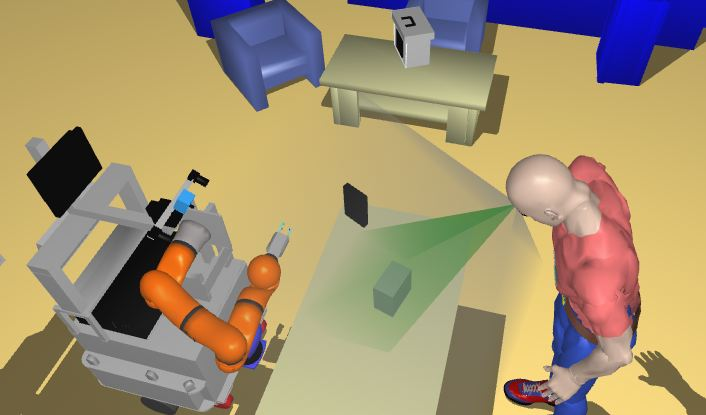
\includegraphics[width=0.4\linewidth]{figs/looks.jpg} 
	}
	\subfigure[]{
		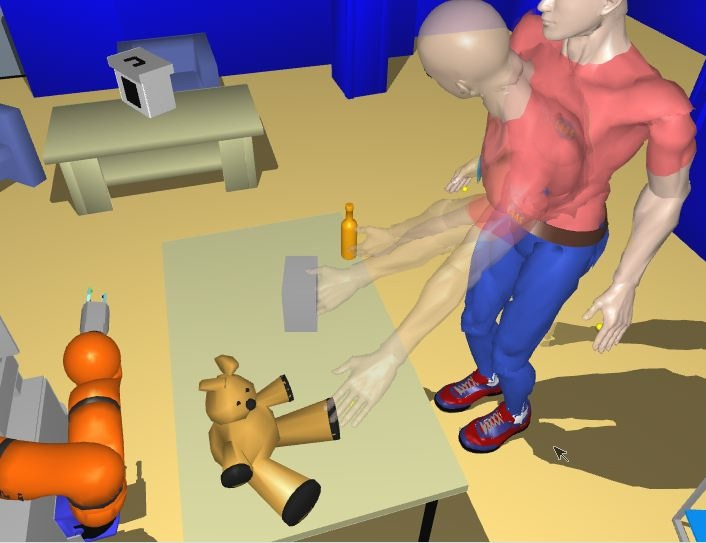
\includegraphics[width=0.35\linewidth]{figs/reach.jpg}
	} 
	\caption{(a) Field of view (FOV) and the field of attention (FOA) of the human. (b) Different reaching postures for the human.}
	\label{fig::sparkRepresentations}
	\end{center}
\end{figure*} 


While the first three relations (\concept{sees}, \concept{looksAt} and
\concept{pointsAt}) are computed through a model based approach, the latter one
is based on the Generalized Inverse Kinematics with pseudo inverse
method~\cite{Nakamura90,Baerlocher04} to find a posture for the
agent where its end-effector is at the center of the object within a given
tolerance.

Tables~\ref{facts|capabilites} summarizes the predicates produced by SPARK
during the agent capabilities analysis phase.

\begin{table}[h]
	\centering
		\begin{tabular}{p{2cm}p{4.5cm}p{2cm}p{3.5cm}}
		\rowcolor{white}
		\textbf{Subject} & \textbf{Predicate} & \textbf{Object} & \emph{Notes} \\
		\hline
		 \concept{Agent}  & \concept{looksAt}  & \concept{SpatialThing} \\
		 \concept{Agent}  & \concept{sees}  &  \concept{SpatialThing}  &    \\ 
		 \concept{SpatialThing}  & \concept{isInFieldOfView}  &  \concept{xsd:boolean}  & via inference: \par \stmt{myself sees *} $\Leftrightarrow$ \stmt{* isInFieldOfView true} \\ 
		 \concept{Agent}  & \concept{pointsAt} $\equiv$ \concept{cyc:pointingToward}  & \concept{SpatialThing} \\ 
		 \concept{Agent}  & \concept{focusesOn}  &  \concept{SpatialThing}  &  via inference: \par \concept{looksAt} $\wedge$ \concept{pointsAt} $\Rightarrow$ \concept{focusesOn} \\
		\concept{Agent} & \concept{seesWithHeadMovement} &  \concept{SpatialThing} \\
		\concept{Agent} & \concept{reaches} &  \concept{Object} \\ 

	\end{tabular}

	\caption{List of facts describing the attentional state and the abilities
	of an agent. \concept{looksAt} is interpreted as an object \emph{being in
	the field of attention} of an agent. An object is \concept{see}n if it is
	visible for the agent without moving the head (\ie, in \emph{field of
	view}).}

	\label{facts|capabilites}
\end{table}

Table~\ref{facts|agentstate} lists the other symbolic facts that are
produced and maintained by SPARK related to the general state of the agent.

\begin{table}[h]
	\centering
	\begin{tabular}{p{2cm}p{5cm}p{2cm}}
		\textbf{Subject} & \textbf{Predicate} & \textbf{Object} \\
		\hline
		\concept{Agent} & \concept{hasIn\{Left|Right\}Hand}  &  \concept{GraspableObject} \\ 
		\concept{Agent} & \concept{hasPosture}  &  \concept{Posture} \\
		\concept{Agent} & \concept{currentlyBodilyDoes}  &  \concept{Action}
	\end{tabular}

	\caption{List of statements describing the state of an agent in general.
	\concept{Posture} can be either \concept{standing} or \concept{sitting}.
	The \concept{currentlyBodilyDoes} predicate states the current action of
	the agent, be it intentional or not.}

	\label{facts|agentstate}
\end{table}


% \begin{table}[h]
% 	\centering
% 	\begin{tabular}{p{2cm}p{5cm}p{2cm}}
% 		\textbf{Subject} & \textbf{Predicate} & \textbf{Object} \\
% 		\hline
% 		\concept{Agent} & \concept{currentlyPerforms})  &  a action \par (\concept{Action})
% 	\end{tabular}
% 	\caption{List of facts describing the current state of a robot.}
% \end{table}

\subsection{Primitive action recognition}
\label{sec|primitives}

Monitoring human activity is crucial to maintain a coherent state of the world.
Full human action and activity monitoring is a difficult task that requires
knowledge and reasoning both on high level facts like goals, intentions and
plans, as well as bottom-up data from agent and object motions. However, simple
temporal and geometric reasoning on human hand trajectories and potential
objects placements can provide some useful clues for high level human
monitoring processes. We call this temporal and geometric reasoning
\emph{primitive action recognition}.

For example, a \emph{pick} or a \emph{throw} action can be
recognized by observing that an object on table and an empty human hand are
close to each other, or that the human hand holding an object is close to a
container, etc. Human hand position is either directly perceived or inferred
from its initial perceived trajectory.  We have a simple implementation of such
a primitive action recognition in SPARK that relies on monitoring a human hand
and its motion near objects or above containers.


%%%%%%%%%%%%%%%%%%%%%%%%%%%%%%%%%%%%%%%%%%%%%%%%%%%%%%%%%%%%%%%%%%%%%%%%%%%%

\subsection{Mightabilities: pro-active analysis of potentialities}

Until now, we have presented techniques to assess, from different perspectives,
the \emph{current} state of the world.

Making effective decisions also requires the ability to assess possible \emph{future}
actions, not only for the robot (by the mean of geometric and/or symbolic planning --
we present in section~\ref{sec|hatp} an example of a symbolic task planner), but
also for the human.

This section explains how potential manipulation actions can be computed for
the human and represented as so-called \emph{Mightability Maps}~\cite{Pandey2010}.

In human movement and behavioral psychology literatures, different types of
reach actions (Fig.~\ref{fig|reaches_taxonomy}) of the human have been
identified and analyzed, \cite{Gardner2001, Choi2004}.

\begin{figure}
  \centering
  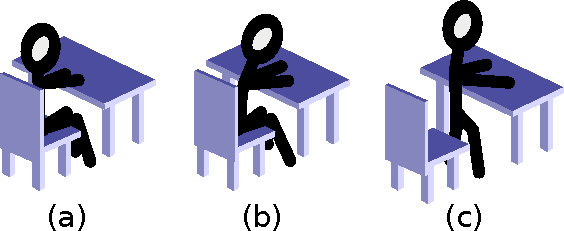
\includegraphics[width=0.7\textwidth]{./figs/reach_postures.pdf} \\
  \caption {Taxonomy of reach actions:(a) arm-shoulder reach, (b) arm-torso 
  reach, (c) standing reach.}
  \label{fig|reaches_taxonomy}
\end{figure}

Taking inspiration from such studies, we introduce the concept of
\emph{mightability}, which stands for ``Might be Able to...'', as a framework
for \emph{multi-state visuo-spatial} perspective taking. The idea is to analyze
the various abilities of an agent such as ability to see or ability to
reach, not only from the current state of the agent, but also from a set of
states, which the agent might achieve from his current state. To this end,
the robot applies a list $A_v$ of virtual actions to estimate the abilities
$A_b \in \{See, Reach, Grasp\}$ from the resulting virtual pose, also
considering the environmental and postural constraints of the agent.

Currently,

\[ 
A_v \subseteq \{A_v^{head}, A_v^{arm}, A_v^{torso}, A_v^{posture}, A_v^{displace}\}
\]

with

\begin{align*}
A_v^{head} & \subseteq \{PanHead, TiltHead\} \\
A_v^{arm} & \subseteq \{StretchOutArm\} \\
A_v^{torso} & \subseteq \{TurnTorso, LeanTorso\} \\
A_v^{posture} & \subseteq \{Stand, Sit\} \\
A_v^{displace} & \subseteq \{MoveTo\} \\
\end{align*}

When such mightability analyses are performed at the levels of cells of the
discretized 3D workspace, we term them as \emph{Mightability Maps} and when done
for the object in the space we call it \emph{Object Oriented Mightabilities}.

The robot performs mightability analyses by taking into account collision as
well as the joint limits. The information about the robot and human positions,
orientations and the 3D state of the environment is continuously updated in the
3D representation and planning platform, Move3D, which also
provides intra-body and inter-body collisions checking for the robot and for
the human models. The robot uses the kinematic structures of the agents and
performs various virtual actions until the joint limits of the neck and/or
torso are reached or the collision of the torso of the agent with the
environment is detected (Fig.~\ref{fig|mightabilities}).

\begin{figure}[ht!]
   \begin{center}
%
       \subfigure[Initial model.]{%
           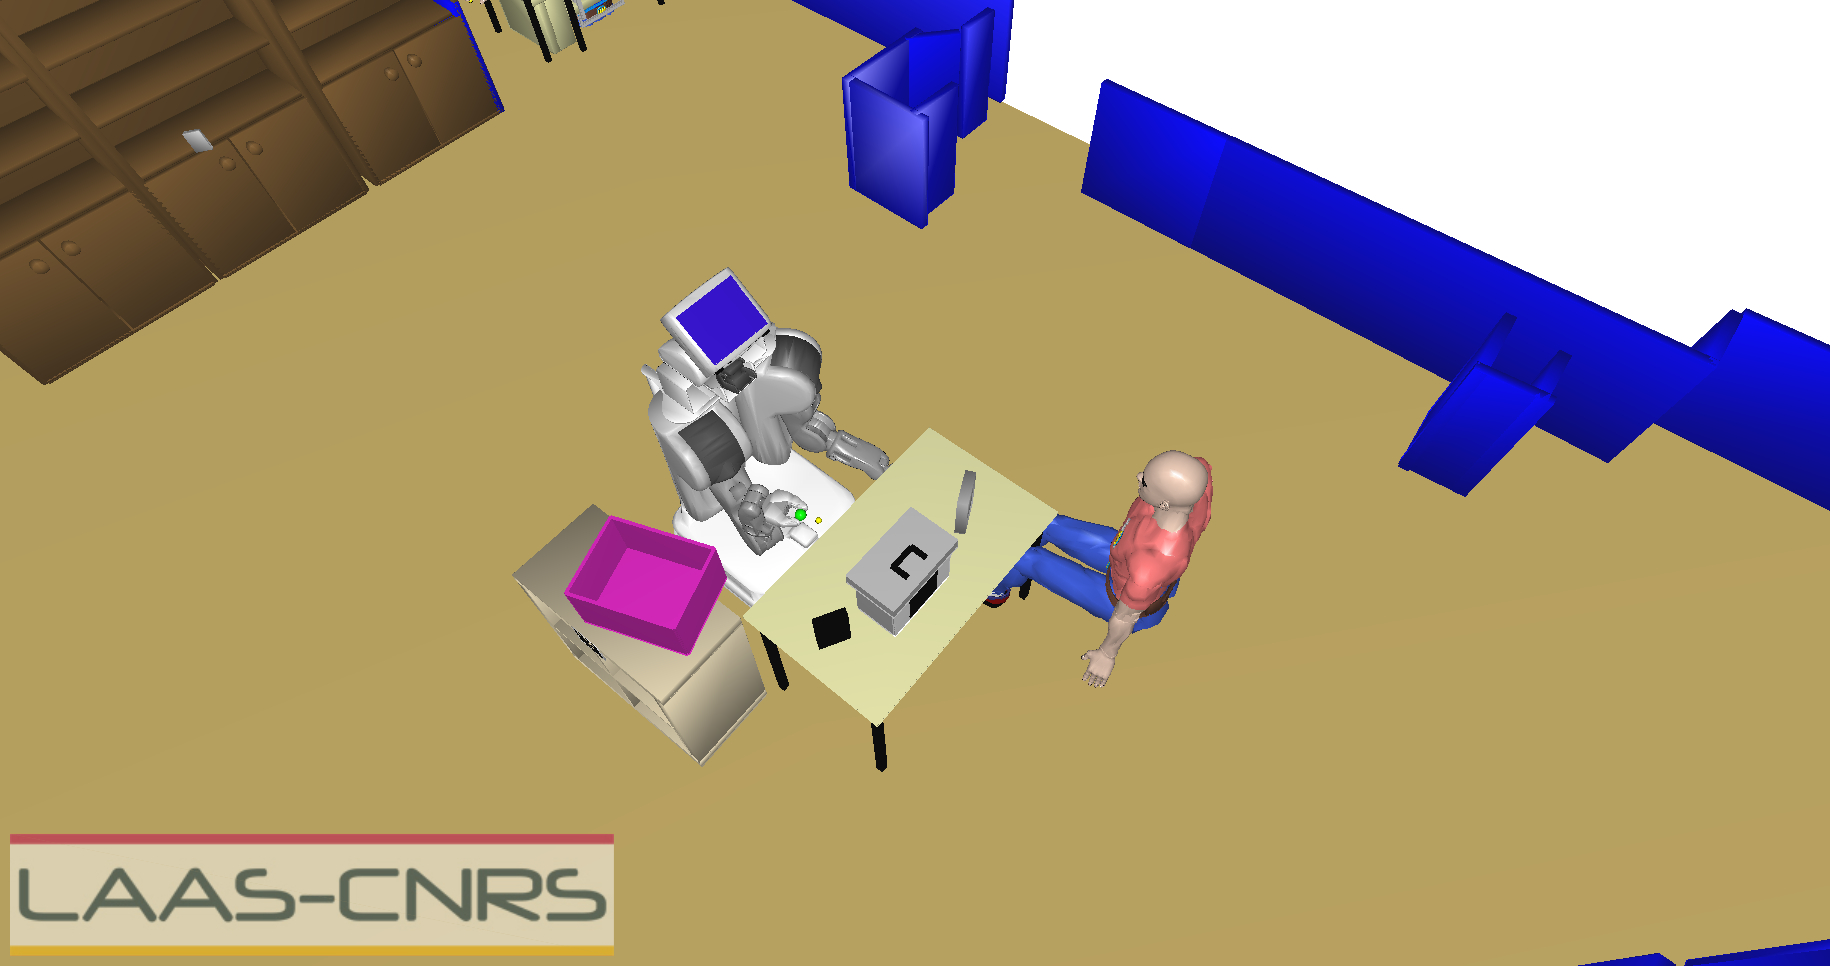
\includegraphics[width=0.5\textwidth]{./figs/mightabilities/2a.jpg}
       }%
	   \subfigure[Mightability Map for the \emph{see} ability. In dark blue,
	   the current field of view, in light green the potential field of view if
	   the human turns his head.]{%
          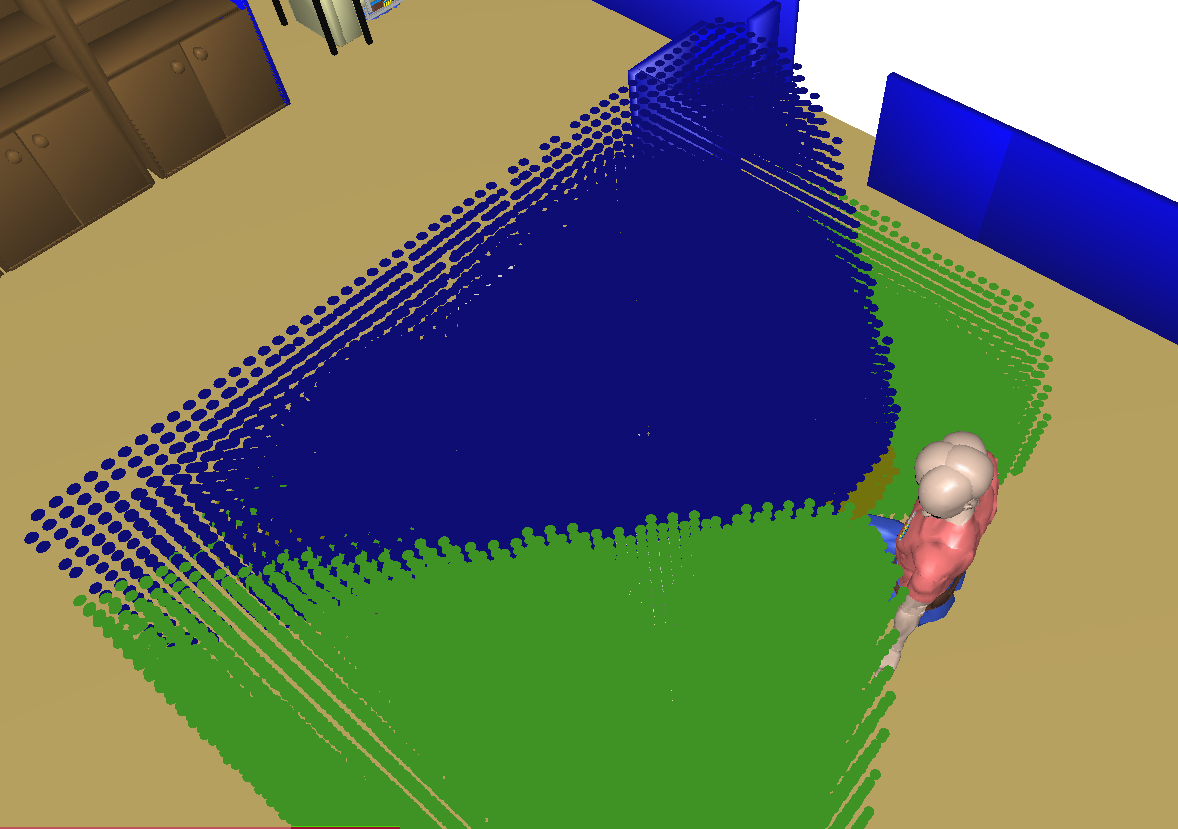
\includegraphics[width=0.5\textwidth]{./figs/mightabilities/2d.jpg}
       }\\%

	   \subfigure[The \emph{reach} ability. In light green, accessible zones if
	   the human leans forward.]{%
          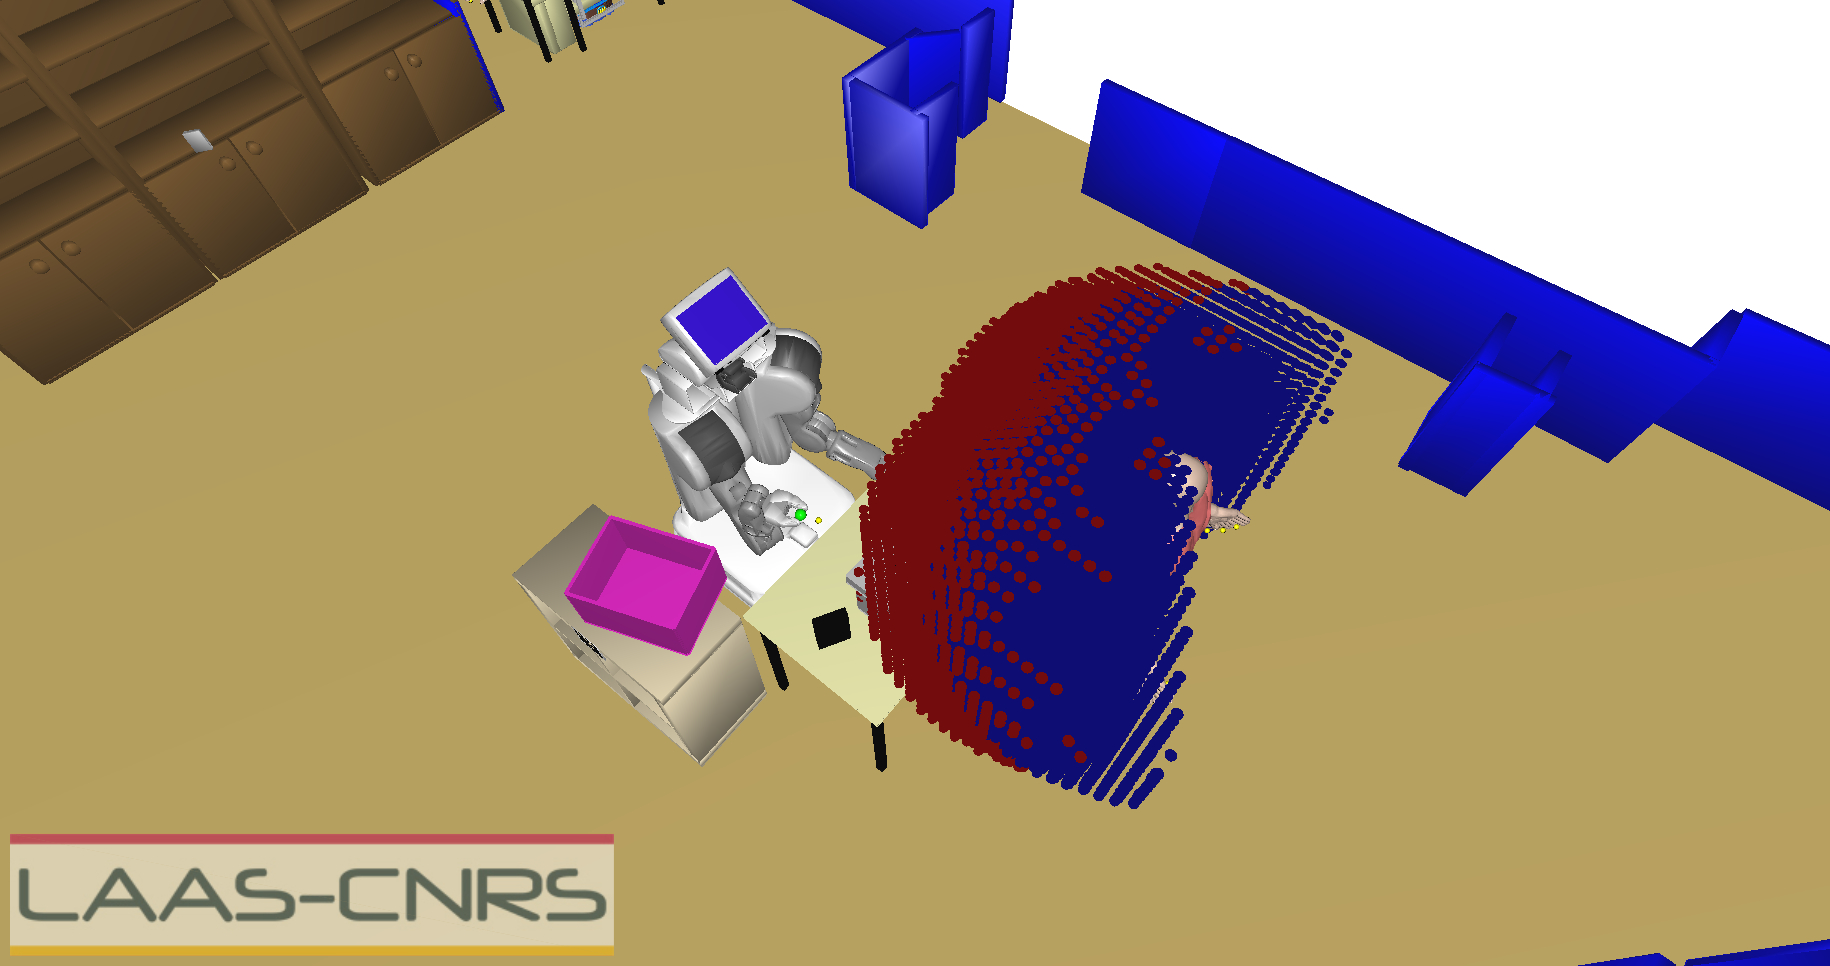
\includegraphics[width=0.5\textwidth]{./figs/mightabilities/2e.jpg}
       }%  
	\end{center}

   \caption{%
	   Examples of a subset of Mightability Maps for the \emph{see} and
	   \emph{reach} abilities.  
	}
		
   \label{fig|mightabilities}
\end{figure}

Thanks to multi-state perspective taking, the robot is also able to estimate
that if the human will just turn his head around, he will be able to see more
places and if the human will lean forward, he will be able to reach more space.
For reachability, the robot further distinguishes among reachable by left hand,
reachable by right hand and reachable by both hands of an agent in a particular
state.  

Mightability analysis can be performed and updated online, making possible to
use it during the planning and decision making steps: as the robot is able to
perform such analysis for all the agents in the environment, it can use the
mightability maps to find the candidate places to perform a set of basic
human-robot interaction tasks: give, make accessible, show, hide an object,
etc. 

\begin{figure}
  \centering
  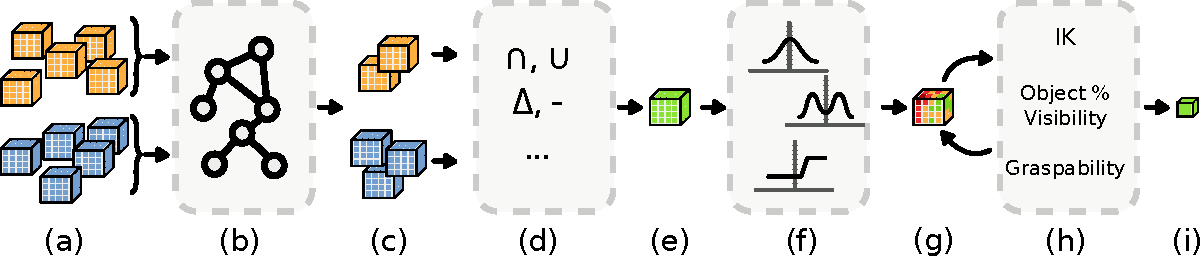
\includegraphics[width=\textwidth]{./figs/mightab-steps.pdf}

\caption {(a) Initial mightability maps, for every agent and evey ability, (b)
Decision making on relevant mightability maps depending on task and required
comfort level of agents, (c) relevant mightability maps, (d) task specific set
operations, (e) raw candidate solution set, (f) weight assignment based on
spatial preferences, (g) set of weighted candidate points, (h) applying
rigorous and expensive tests on reduced search space, (i) the feasible solution
of highest weight.}

  \label{fig|mightabilities-framework}
\end{figure}


Figure~\ref{fig|mightabilities-framework} shows how a feasible solution for a
task can be found: the robot reasons on various mightability maps of the
involved agents and selects the best solution by performing successive set
operations depending on the task.

\begin{figure}[ht!]
   \begin{center}
       \subfigure[]{%
           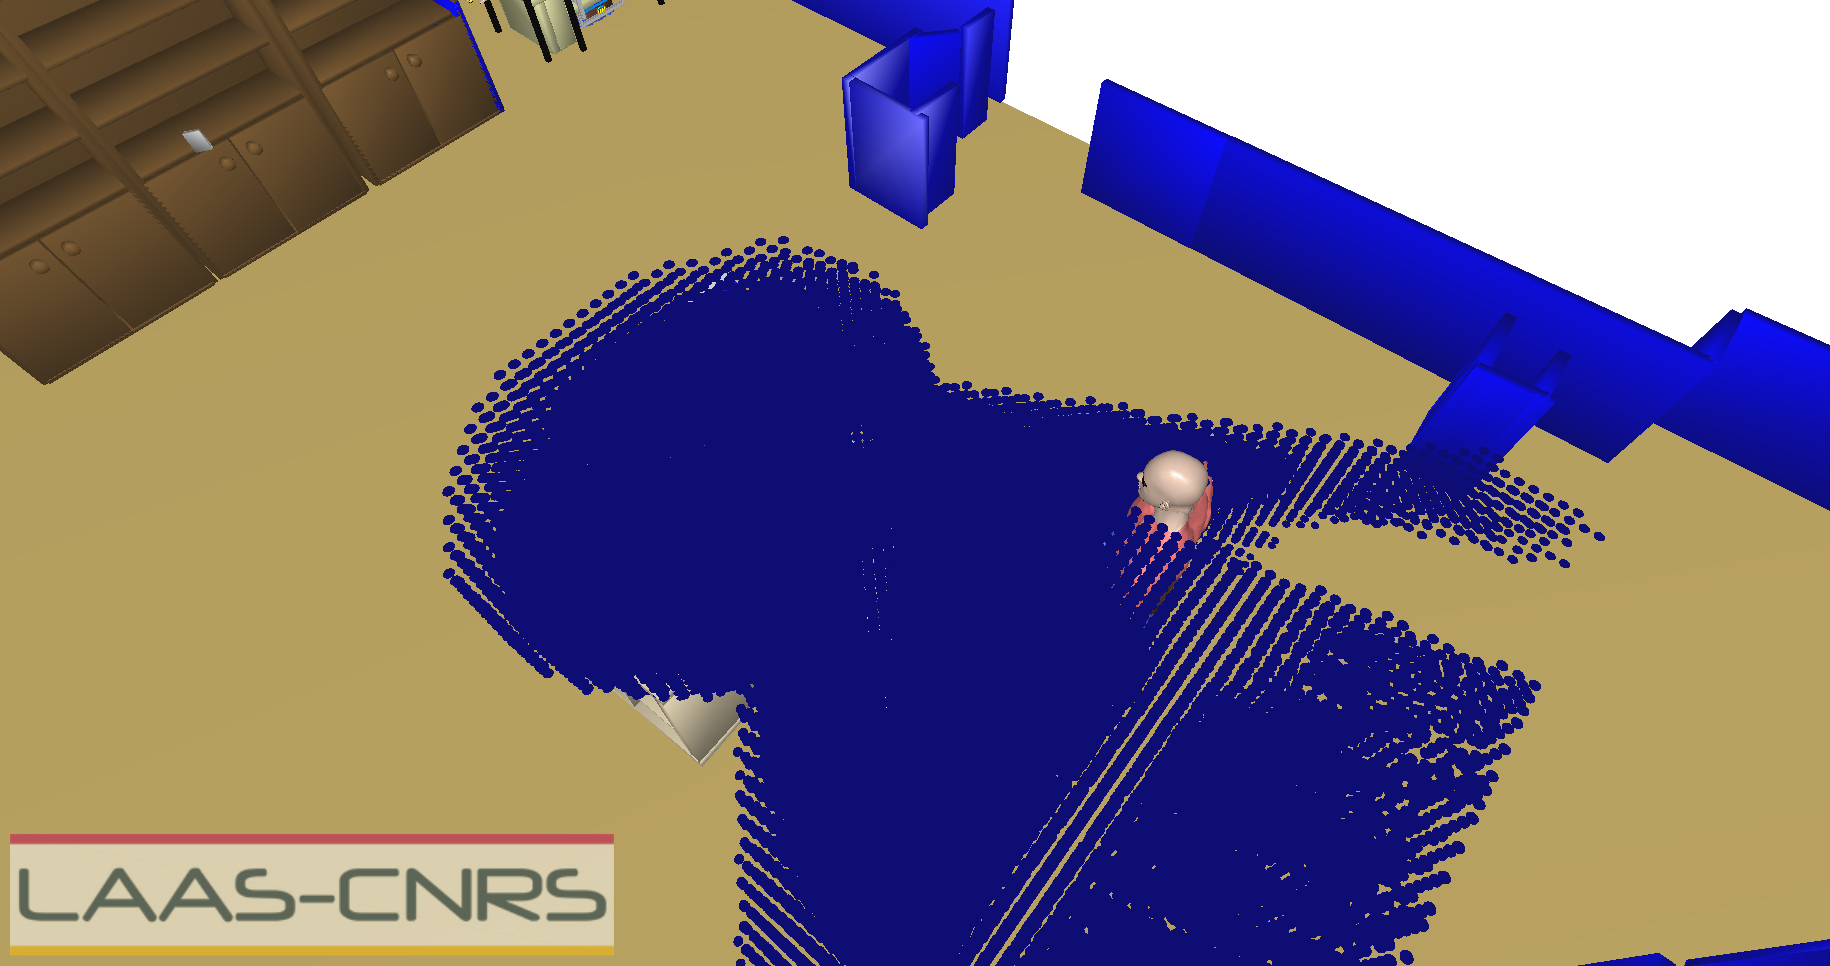
\includegraphics[width=0.5\textwidth]{./figs/mightabilities/4a.jpg}
       }%
       \subfigure[]{%
          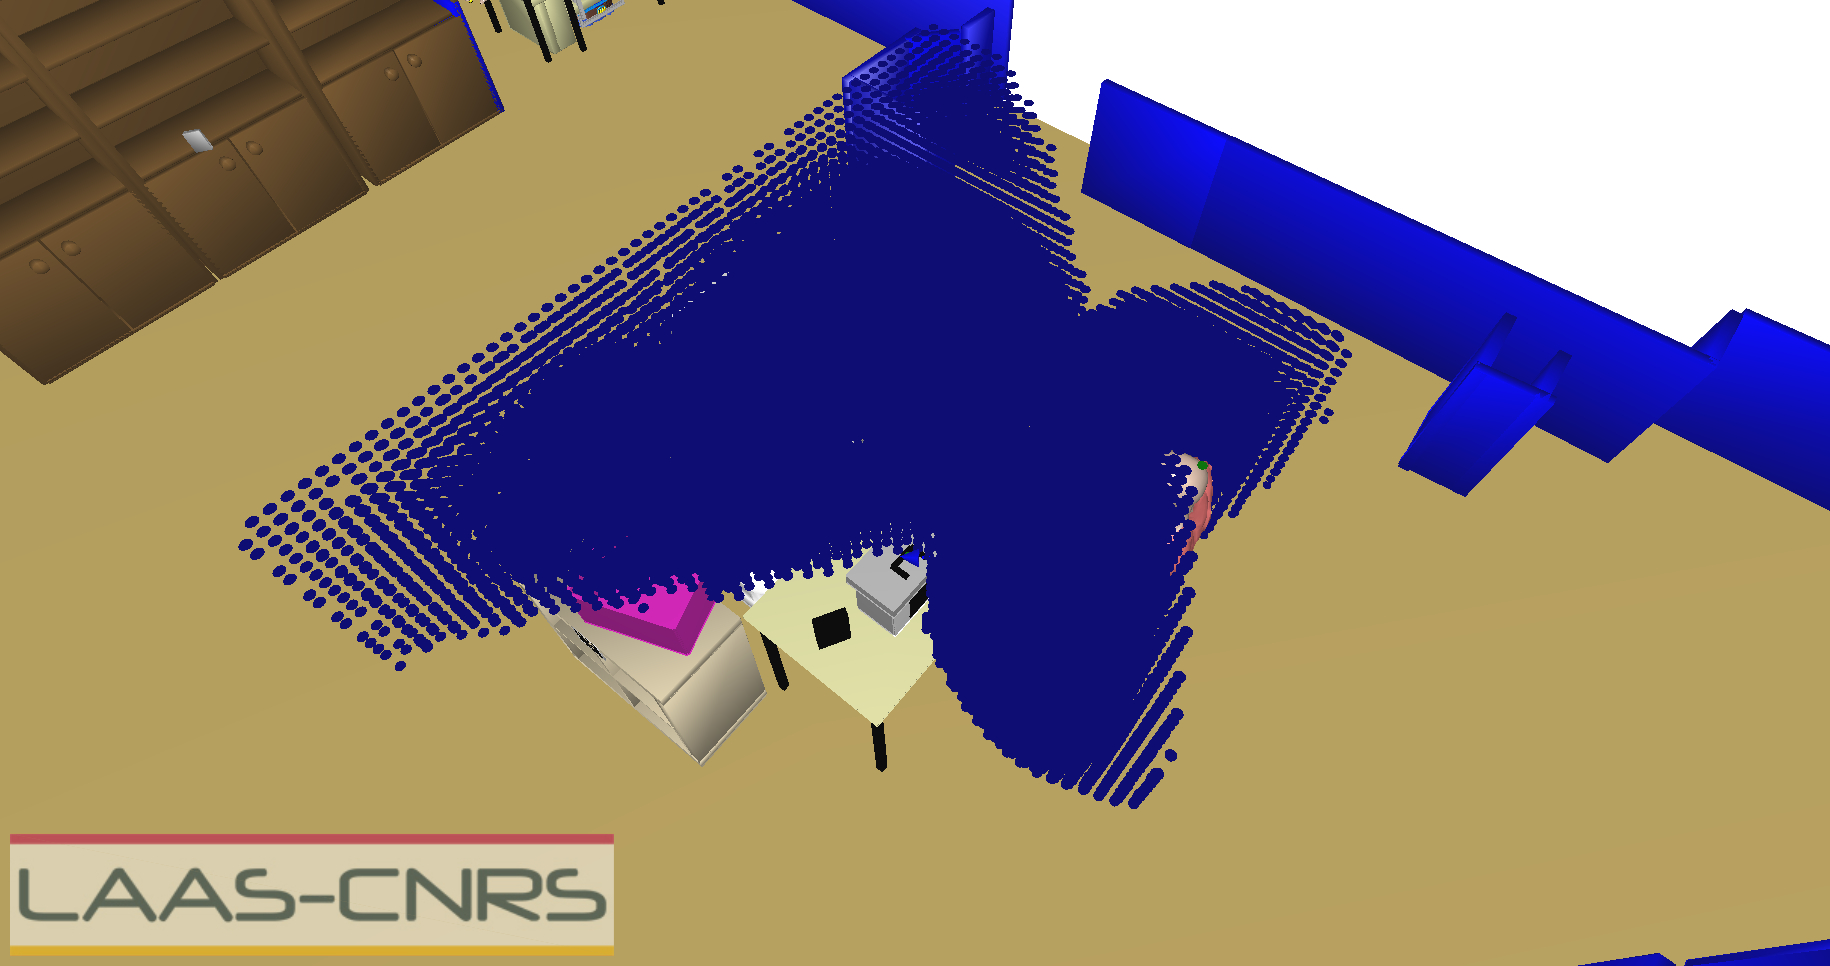
\includegraphics[width=0.5\textwidth]{./figs/mightabilities/4b.jpg}
       }\\ %  ------- End of the first row ----------------------%
       \subfigure[]{%
           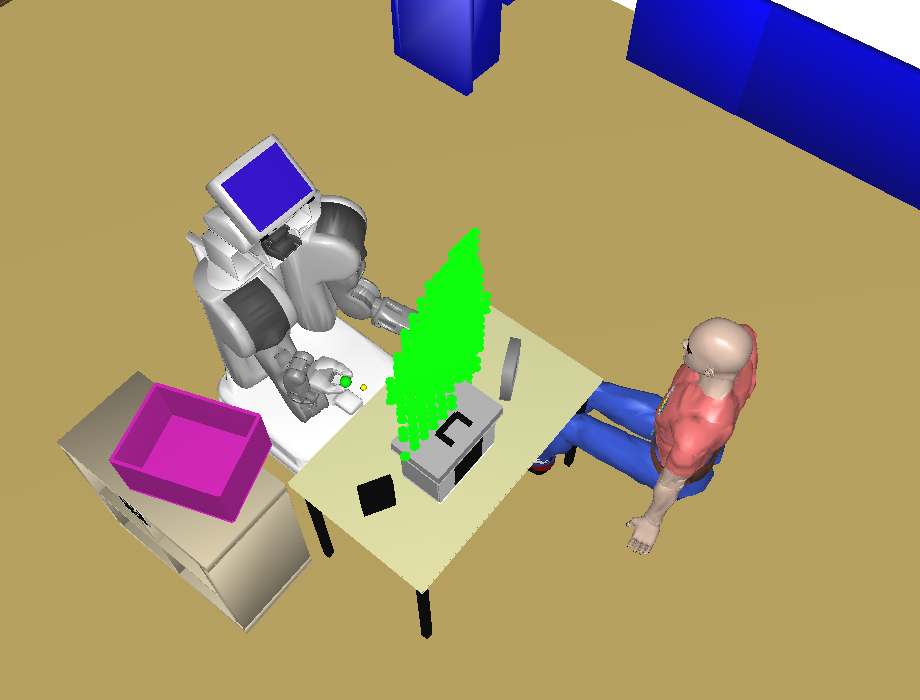
\includegraphics[width=0.5\textwidth]{./figs/mightabilities/4c.jpg}
       }%
       \subfigure[]{%
          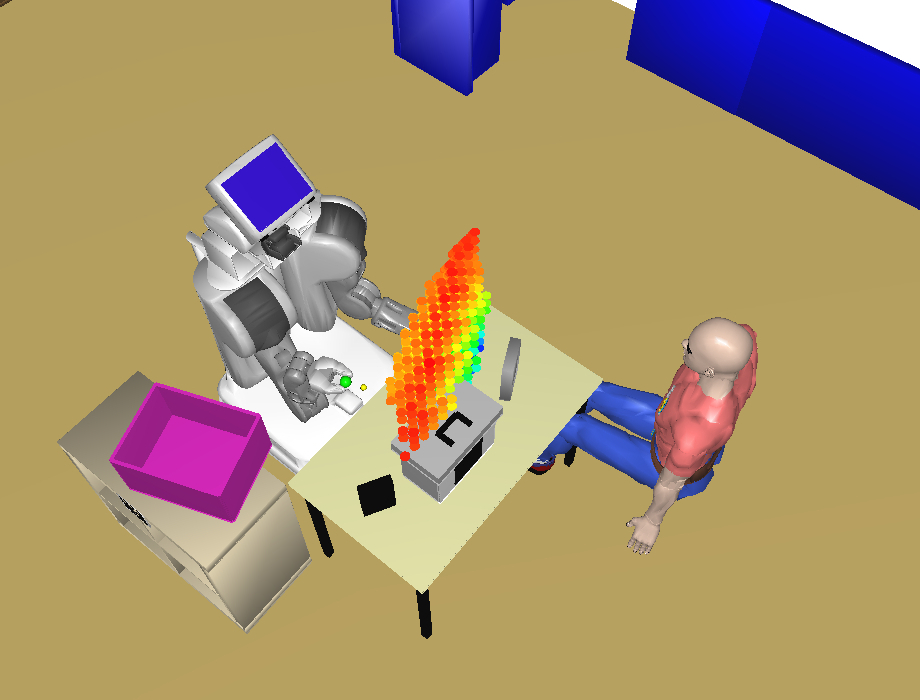
\includegraphics[width=0.5\textwidth]{./figs/mightabilities/4d.jpg}
       }
	\end{center}

   \caption{
	Steps for finding weighted candidate search space for the task of robot
	giving an object to the human. {\it(a)} \emph{sees} and \emph{reach} map
	for the robot, {\it(b)} \emph{sees} and \emph{reach} map for the human,
	{\it(c)} zone visible and accessible for both agents, {\it(d)} weighted
	candidate points}
		
   \label{fig|mightabilities-steps}
\end{figure}

Figure~\ref{fig|mightabilities-steps} illustrates the process for a \emph{give}
task. From the initial set of all the mightability maps for the robot and for
the human, the planner extracts the relevant mightability maps based on the
task and the desired efforts of the agents.

In this example, the maximum desired effort for the human is to lean forward.
As the task requires a hand-over operation, we compute positions visible and
reachable by both agents (Fig.~\ref{fig|mightabilities-steps}{\it c}) from
each agent's respective maps (Figs.~\ref{fig|mightabilities-steps}{\it a} and
{\it b}).

Further based on various criteria such as comfort, preferences, etc. weights
are assigned to the raw candidate points
(Fig.~\ref{fig|mightabilities-steps}{\it d}), and the resulting candidates are
iteratively tested for feasibility by introducing computationally expensive
constraints such as existence of a collision-free trajectory.

\subsection{Related work}

Breazeal et al.~\cite{breazeal2006} present a learning algorithm that takes
into account information about a teacher's visual perspective in order to learn
a task.  ~\cite{Johnson2005} apply visual perspective taking for action
recognition between two robots.~\cite{Trafton2005} use both visual and spatial
perspective taking for finding out the referent indicated by a human partner.

%%%%%%%%%%%%%%%%%%%%%%%%%%%%%%%%%%%%%%%%%%%%%%%%%%%%%%%%%%%%%%%%%%%%%%%%%%%%
%%%%%%%%%%%%%%%%%%%%%%%%%%%%%%%%%%%%%%%%%%%%%%%%%%%%%%%%%%%%%%%%%%%%%%%%%%%%

\section{Explicit Knowledge Management}
\label{cognitivekernel}

The previous sections have presented how symbolic facts, grounded in the
current physical situation, were generated by the robot. This section now
presents how we store and reason about these symbolic statements.

\subsection{Ontology-based Knowledge Management}

A key element of this cognitive architecture is how knowledge is explicitly
exposed, stored and handled between components.

We have adopted a centralized approach for knowledge management called
ORO~\cite{Lemaignan2010}. The platform is designed as a central knowledge
storage service implemented as a server where the robot components can add or
query statements at run-time. Figure~\ref{fig|oro-overview} illustrates the
main functional components of ORO.

\begin{figure}
\centering
  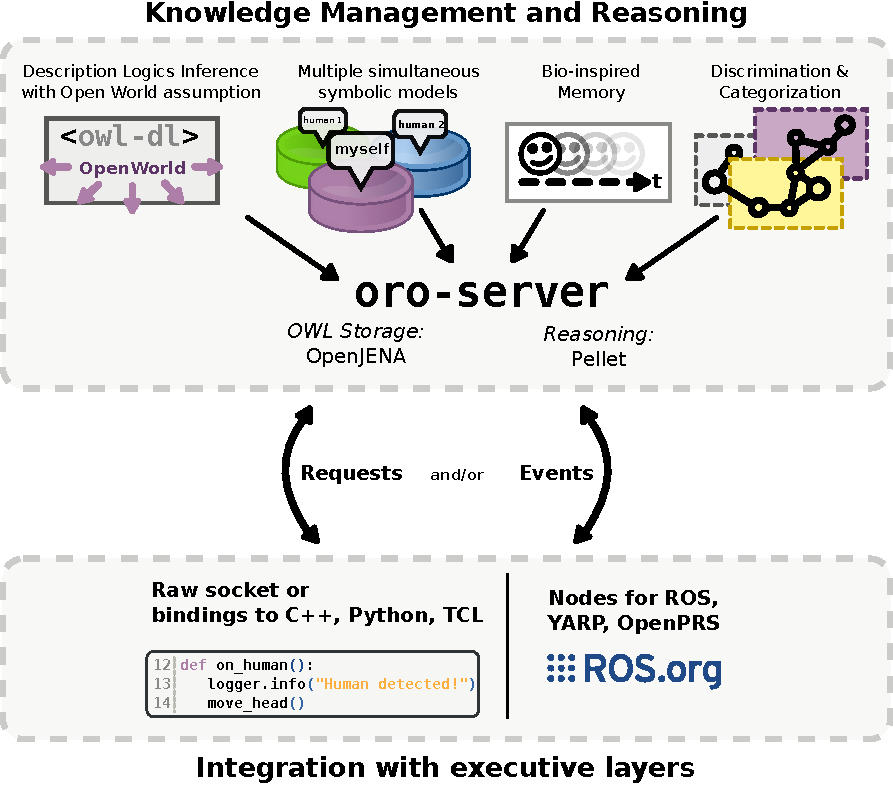
\includegraphics[width=0.8\linewidth]{figs/oro_architecture_functional.pdf}
  \caption{Overview of the ORO architecture.}
  \label{fig|oro-overview}
\end{figure}

At the core, ORO is build around the
OpenJena\footnote{\url{http://www.openjena.org}} ontology management library,
connected to the Pellet\footnote{\url{http://clarkparsia.com/pellet}} reasoner.

A front-end accepts and manages connections to clients. The clients' requests
are processed by a set of internal modules: basic operations on statements, but
also higher cognitive and human-robot interaction related functionalities are
available. External plugins can also be easily added.

Besides acting as a facts database, the ORO platform exposes several functions:
operations on knowledge statements relying on inference (through a continuous
first-order logic classification process), management of \emph{per-agent}
symbolic models, and also higher cognitive and human-robot interaction related
functionalities like categorization of sets of concepts or profiles of memory
(that enable the robot to ``forget'' about some facts).

ORO also provides an event mechanism that allows components to be
triggered when specific events occur. A component can
for instance subscribe to events of kind \setstmt{?agent isVisible
  true, ?agent type Human}. As soon as the perception layer detects a
human in the robot's field of view and accordingly updates the
knowledge base, the executive layer is triggered. The
event framework also takes advantage of the inference capabilities of
ORO. Thus an event can be indirectly triggered if its triggering
conditions can be inferred to be true.

\subsection{Common-Sense Knowledge}
\label{ontology}

For the robot to interpret and come up with new inferences based on the facts
coming from the perceptual layers, it needs a \emph{cultural background}, a
common-sense knowledge assumed to be shared by all agents. The ORO server is
loaded at startup with an initial set of statements which we call the
\emph{OpenRobots Common Sense Ontology}. It defines concepts
(and implicitly, a vocabulary) that can be used by all the modules of the robot
to unambiguously add or query facts. Moreover, the same ontology declares rules
and logical properties that are later on used for inference.

The \emph{OpenRobots Common Sense Ontology} defines a small set of classes (56
are currently defined) and predicates (60 are currently defined) focused on
concepts useful for human-robot interaction. It includes both very broad
categories like \concept{SpatialThing}, \concept{Event} or \concept{Action},
and much more concrete concepts as \concept{Table}, \concept{Book} or colors.
Available predicates allow us to describe the state of the agents and the world
with relations like \concept{isOn}, \concept{sees},
\concept{currentlyPerforms}, etc.

Our common sense ontology is closely aligned with the open-source
OpenCyc\footnote{\url{http://www.opencyc.org}} upper ontology.  OpenCyc defines
a large taxonomy of concepts and semantic relationships between concepts that
are used in several other projects (\textsc{WordNet, DBpedia}). This
potentially eases the exchange and addition of knowledge from these other
sources. It also enables knowledge exchange with other robots (for instance,
the work by Daoutis~\cite{Daoutis2009} or Tenorth~\cite{Tenorth2009a} are also 
aligned on Cyc concepts).

\subsection{Reasoning and Dynamic Knowledge Structuring}

Knowledge is stored as OWL/RDF ontologies in ORO. We use the Pellet reasoner to
classify them. This enables several type of reasoning:

\begin{itemize}
	\item reasoning on inheritance relations (\eg \emph{all bottles are containers}),
	\item property axioms
		\begin{itemize}
		\item entailments based on predicates' domain and range,
		\item cardinality constraints (including \concept{allValue}, 
		\concept{someValue}, \concept{hasValue}),
		\item property characteristics (symmetry, transitivity)
		\end{itemize}
	\item class restrictions like: \par \footnotesize \concept{Bottle} $\equiv$
		\concept{Artifact} {\bf that} (\concept{hasShape} {\bf value}
		\concept{cylinderShape})\footnote{This example uses the \emph{Manchester
		syntax}, \url{http://www.w3.org/TR/owl2-manchester-syntax/}} \normalsize
	\item set operations like: \par \footnotesize \concept{Color} $\equiv$ {\bf unionOf}(\concept{blue},
		\concept{green}, \concept{orange}, \concept{black}...) \normalsize
	\item generic SWRL ({\em Semantic Web Rule Language}) rules like: \par
		\footnotesize \concept{looksAt(?agt, ?obj)} $\land$
		\concept{pointsAt(?agt,?obj)} \par $\Rightarrow$ \concept{focusesOn(?agt, ?obj)}
		\normalsize 
	\end{itemize}

We provide in ORO accessors to query, add or remove all these properties and
restrictions (except the SWRL rules) at run-time. This allows knowledge
introspection and enables the robot to alter its own knowledge structures (the
so-called \emph{T-Box} model) during its life-time by adding new constraints
and properties to classes and predicates (we can for instance teach the robot
\emph{at runtime} that cats are animals, \ie \stmt{Cat rdfs:subClassOf
Animal}).

\subsection{Representation of Alternative Cognitive Models}
\label{alterite}

As pictured in Fig.~\ref{fig|oro-overview}, ORO stores independent cognitive
models for each agent it interacts with. When ORO actually identifies a new
agent (or infers that some instance is an agent), it automatically creates a
new, separate, in-memory OWL model for that agent. Thus, different robot
components, like execution control or situation assessment, can access the
agents' beliefs in separate models. All knowledge processing functions in the
robot's primary model are equally available in every agent's model.

Each of these models is independent and logically consistent,
enabling reasoning on different perspectives of the world that would otherwise
be considered as globally inconsistent (for instance, an object can be visible for the
robot but not for the human. This object can have at the same time the property
\concept{isVisible \textbf{true}} and \concept{isVisible \textbf{false}} in
two different models). 

This feature actually allows us to consider the robot to be endowed with a partial
\emph{theory of mind}~\cite{Leslie2000}: the robot can explicitly model
the belief states of its interactors, opening new possibilities for the control
architecture. In section~\ref{dialogs} we present an example of how we use this feature to
make sense of user sentences from his/her point of view.

% \subsection{Categorization}
% \label{categorization}
% 
% We have implemented several algorithms (common ancestors, computation of the
% best discriminant~\cite{Ros2010b}) to help the robot cluster a set of
% concepts based on their symbolic similarities. One particular application of these functions is discrimination.
% While interacting with a user, the robot quite often needs to clarify an
% ambiguity produced by its human partner. For instance, a user may refer to a
% ``bottle'' where two bottles are currently visible. Discrimination routines
% can identify possible (symbolic) differences (\eg the color or the size of the
% bottles) that permit the robot to ask an accurate question to the user in order
% to solve the ambiguity. This discrimination can occur from the robot's
% perspective or from a specific agent's perspective. Usage of these
% categorization abilities are illustrated in Sections~\ref{dialogs:disamb} and~\ref{spygame}.
% 


\subsection{Related work}

Knowledge representation systems are always present in some form in robotic
architectures that claim to be somehow \emph{cognitive}. While centralized
knowledge bases are the most common approach in the literature, other, more
pervasive, approaches exist, like \cite{Jacobsson2008}.

We mention only two of them here. Other systems that are part of larger
architectures for grounding of human-robot interaction are presented in
section~\ref{sec|literature}.

In the field of symbolic knowledge processing for robots, Gunderson and
Gunderson~\cite{Gunderson2008} introduce the concept of \emph{reification}
(based on both recognition and pre-afference) as an intermediate step between
pattern recognition and symbol grounding. Their underlying storage of knowledge
relies on ontologies and bio-inspired memory models.

Beetz et al.~\cite{Beetz2010} proposes a cognitive architecture called
\textsc{CRAM} (Cognitive Robot Abstract Machine) that integrates
\textsc{KnowRob}~\cite{Tenorth2009a}, a knowledge processing framework based on
Prolog. Its underlying storage is based on an OWL ontology, derived from
\textsc{OpenCyc}. \textsc{CRAM} and \textsc{KnowRob} have been demonstrated on
several real-world scenarios, where natural language recipes extracted from the
Internet had to be translated into plans and executed in a kitchen environment,
perceived and rebuilt on-line by the robots. While Prolog offers more flexible
modeling (no constraints on the arity of predicate, where Description Logics as
used in our work are limited to binary predicates), it is based on the closed
world assumption (if something cannot be inferred to be true, it is inferred to
be false) whereas we rely on the open world assumption, which is more realistic
in real world scenarios. A probabilistic extension of \textsc{KnowRob}, called
\textsc{ProbCog}~\cite{Jain2009} is also available. While in principle
possible, currently the CRAM architecture does not provide explicit support for
interacting with humans.

On the topic \emph{common-sense knowledge}, several significant projects are
trying to provide a machine-processable repository of common sense facts
produced by humans (the \textsc{OpenMind} project~\cite{Singh2002} or
RoboEarth~\cite{Waibel2011} are --very different-- examples). These knowledge
bases are valuable but remain sometimes difficult to use in a pervasive way
because of both their incompleteness and the lack of good connections with
underlying, unambiguous concepts.


%%%%%%%%%%%%%%%%%%%%%%%%%%%%%%%%%%%%%%%%%%%%%%%%%%%%%%%%%%%%%%%%%%%%%%%%%%%%
%%%%%%%%%%%%%%%%%%%%%%%%%%%%%%%%%%%%%%%%%%%%%%%%%%%%%%%%%%%%%%%%%%%%%%%%%%%%

\section{First Application: Goal and Plan Management}
\label{sec|hatp}

Complex human robot interaction may necessitate a strong reasoning about
the environment and the capabilities of involved agents: How can they
achieve a specific goal? What are the required actions to achieve this
goal? Which actions can be performed by each agent? etc.

In the previous sections, we have seen how symbolic knowledge is produced
and stored from the real physical world. In this section, we present one
possible way to use these symbolic models of the environment and
interacting agents to produce a plan of actions for a complex
goal.

In order to devise how a given goal can be accomplished, the robot has
to elaborate a plan,\ie a set of actions to be achieved by
the robot and its human partners.  This is the role of HATP
\cite{Alili2008} (for Human Aware Task Planner).  HATP is based on a
Hierarchical Task Network (HTN) refinement, which performs an iterative
task decomposition into sub-tasks until reaching atomic
actions~\cite{Nau2003}.  The planning domain defines a set of methods
describing how to decompose a task and can be seen as the {\it how-to}
knowledge of the robot.  HATP is able to produce plans for the robot's
actions as well as for the other participants (humans or robots). It
can be tuned by setting up different costs depending on the actions to
apply and by taking into account a set of constraints called social
rules. This tuning aims at adapting the robot's behavior according to
the desired level of cooperation of the robot.

\subsection*{Agents and action streams}

The robot plans not only for itself but also for the other agents. The
resulting plan, called ``shared plan'' is a set of actions that form
a stream for each agent involved in the goal achievement. Depending on
the context, some ``shared plans'' contain causal relations between the
agents. For example, the second agent needs to wait for the success of
the first agent's action to be able to start its own action. When the
plan is performed, causal links induce synchronization between
agents. Figure~\ref{plan_hatp1} illustrates a plan with two streams.

\begin{figure}[htbp]
  \centering
  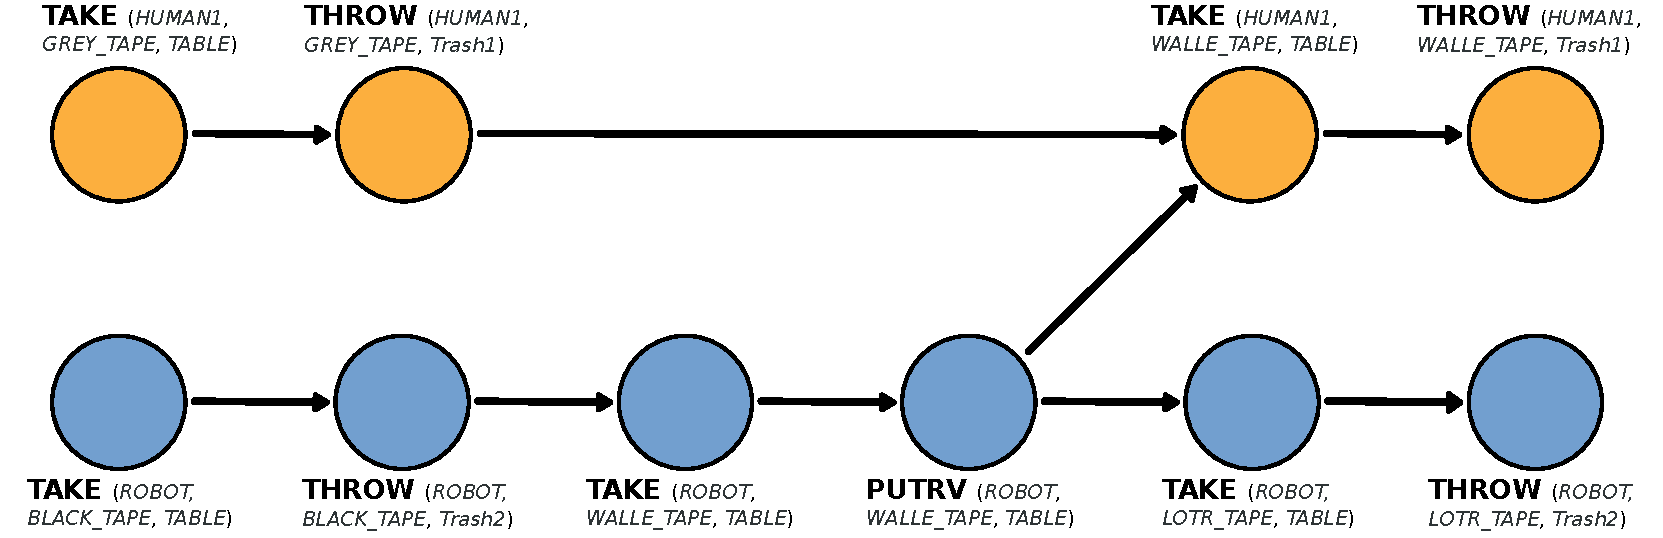
\includegraphics[width=0.95\columnwidth]{./figs/plan1.pdf}
  \caption{A plan produced by HATP with 2 streams}
  \label{plan_hatp1}
\end{figure}

\subsection*{Action costs and social rules}

A cost and a duration function is associated to each action.  The duration
function provides a duration interval for the action achievement and is used,
in one hand, to schedule the different streams and, in the other hand, as an
additional cost function.  In addition to these costs, HATP also takes into
account a set of social rules.  Social rules are constraints aiming at leading
the plan construction towards the best plan according to some human
preferences. The social rules we have defined so far deal with:

\begin{itemize}
\item undesirable state: to avoid a state in which the human could
  feel uncomfortable;
\item undesirable sequence: to eliminate sequences of actions that can
  be misinterpreted by the human;
\item effort balancing: to adjust the work effort of the agents;
\item wasted time: used to avoid long delays between the actions of
  the human partner;
\item intricate links: to limit dependencies between the actions of
  two or more agents.
\end{itemize}

\begin{figure}[htbp]
  \centering
  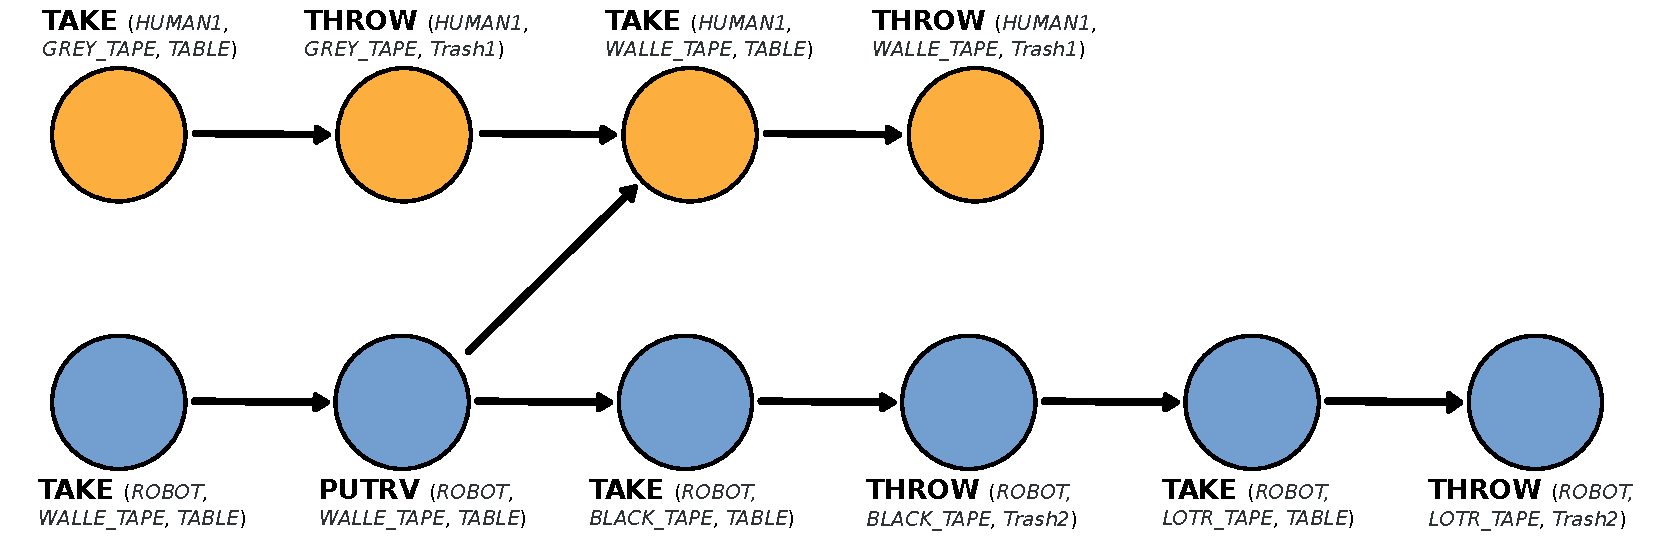
\includegraphics[width=0.95\columnwidth]{./figs/plan2.pdf}
  \caption{A plan with the wasted time social rule}
  \label{plan_hatp2}
\end{figure}

Figure~\ref{plan_hatp2} illustrates an alternative plan to the previous 
one (Fig.~\ref{plan_hatp1}) if the wasted time social rule is used.
The obtained shared plan is the best plan according to a global evaluation of
these multiple criteria.

\subsection*{Several levels of cooperation} 

By tuning its costs and adapting its social rules, HATP can be used to compute
various alternative plans. These plans can be categorized into several levels
of cooperation

\begin{itemize}
\item helping the human to achieve his goal by acting for him
\item sharing concrete resources by handing some objects
\item collaboration of the robot and the human by coordinating their
  actions towards a human-robot joint goal.
\end{itemize}



%%%%%%%%%%%%%%%%%%%%%%%%%%%%%%%%%%%%%%%%%%%%%%%%%%%%%%%%%%%%%%%%%%%%%%%%%%%%
%%%%%%%%%%%%%%%%%%%%%%%%%%%%%%%%%%%%%%%%%%%%%%%%%%%%%%%%%%%%%%%%%%%%%%%%%%%%

\section{Second Application: Natural Language Grounding}
\label{dialogs}

Looking back at our initial example, we wanted to make sense of the utterance
``\emph{Robot, put the two glasses and this bottle on the tray!}''.

The first step is to understand the meaning of the sentence. To this end, we
must acquire the sentence, convert it into a useful syntactic form (usually
through speech recognition), and understand the semantics of the sentence, \ie
What is referred by ``\textit{Robot}''? What is ``\textit{put}''? What are
``\textit{the}''? And ``\textit{two}''? etc.

Working in a situated context, we need to \emph{resolve} these semantics atoms,
\ie group them and ground them in the sensory-motor space of the robot. For instance,
``\textit{this bottle}'' is a demonstrative group that refers in this context to the
bottle the human is focusing on.

The next step is to extract and understand the \emph{intended meaning} of the
utterance as thought by the agent. In our example, the human obviously wants an
action to be performed by the robot. In our example, the type of action is
given by the verb ``\textit{put}''. Assuming the robot has some procedural
knowledge attached to this symbol, the action type can be considered as
grounded for the robot. The action parametrization is conveyed by the semantics
attached to the words and the grammatical structure of the sentence: we
understand that the recipient of the action is the human, the performer is the
robot itself, and the objects acted upon are two glasses and a bottle. The
recipient, the performer and the object are three of the \emph{thematic
roles}~\cite{Gruber1965} that qualify the \emph{put} action. They are necessary
to fully ground the sentence\footnote{This analysis has been inspired on the
work of Austin et al.~\cite{Austin1962}, where this type of sentences
correspond to \emph{speech acts}, comprising of \emph{locutionary act} (the
meaning), \emph{illocutionary} (the intent) and possibly \emph{perlocutionary
acts} (implicit speaker's expectation).}.

To summarize, verbal interaction with human presents two categories of challenges: syntactic
ones, and semantic ones. The robot must be able to process and analyze the
structure of human utterances, \ie natural language sentences, and then make
sense of them. 

In this second application of our cognitive architecture, we show how we
harness the symbolic knowledge base to tackle the semantic challenge: how to
ground and interpret the meaning of verbal instructions.

Note that this process also takes full advantage of the embodied nature of the
interaction: because deictic gestures and postures are also available in the
symbolic knowledge base and dynamically updated during the interactions, verbal
dialogue processing turns into a truly multi-modal communication processing,
leading to more robust interpretation.

\begin{figure}[!t]
\centering
  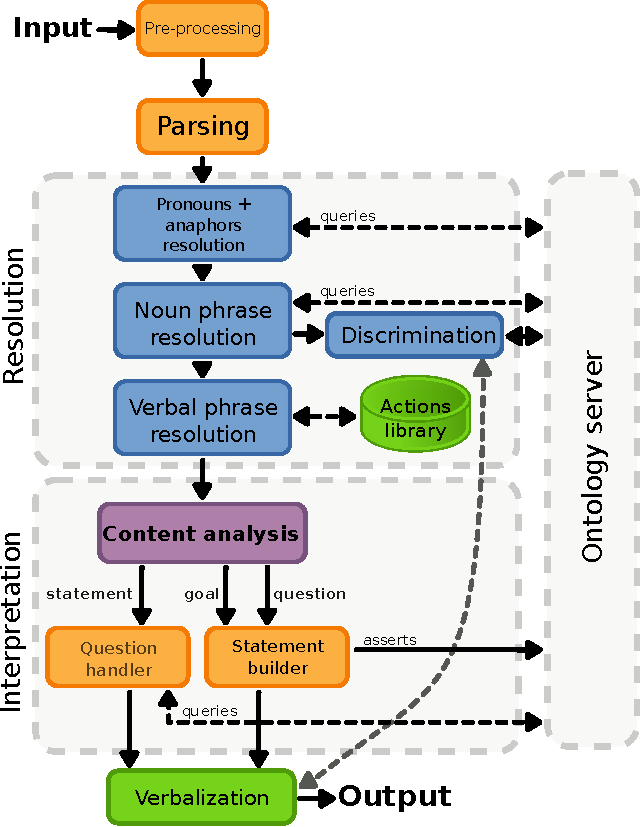
\includegraphics[width=0.5\linewidth]{figs/dialog_module_simple.pdf}
  \caption{The {\sc Dialogs} module has three main steps: the parsing,
  the interpretation and the verbalization. The interpretation module is
  responsible for both the \emph{resolution} and the semantic content
  \emph{analysis and translation}.} 
  \label{fig|dialog}
\end{figure}

Dialogue processing is done in our architecture by a module called {\sc
Dialogs}\cite{Lemaignan2011a} (Fig.~\ref{fig|dialog}) that processes human
input in natural language, grounds the concepts in the robot's knowledge and
eventually translates the discourse in a set of queries or declarative OWL/RDF
statements.  

The user's input is first pre-processed (for instance, \emph{I'm} constructs
are expanded into \emph{I am}) and then parsed by a rule-based (\ie
grammar-free) tool that extracts the grammatical structure from the user's
sentence. Figure~\ref{dialog|parser_output} shows an example of the raw output
of the parser for a moderately complex sentence.

\begin{figure}%[!ht]
\begin{center}
\scriptsize
\begin{alltt}
>> IMPERATIVE
VP: \textbf{remember} (present simple)
    SUBSENTENCE (aim: that)
      NP: \textbf{I}
      VP: \textbf{want} (present simple)
        direct objects: 
          NP: \textbf{you}
        secondary VP: \textbf{give} ()
              direct objects:
                NP: my \emph{nice blue} \textbf{bottle}
              indirect objects:
                NP: \textbf{me}
\end{alltt}
\end{center}
\caption{Raw output of the {\sc Dialogs} parser after processing the
sentence: ``remember that I want you to give me my nice blue bottle.'' 
Grounding has yet to take place.} 
\label{dialog|parser_output}
\end{figure}

The output of the parser is then sent to the \emph{interpretation} module, the
core of the component.  Interpretation consists in three distinct operations:
the sentence \emph{resolution} (concepts grounding), the \emph{content
analysis} (what is the intent of the utterance: information, question or
desire) and the \emph{statement building} (translation into OWL statements).

The sentence resolution has three steps: {\it(i)} pronouns and anaphora are
replaced by the correct speaker ID and the ID of the last object referred to
(extracted from the dialogue history) respectively, {\it(ii)} nominal groups are
disambiguated and grounded (noun phrase resolution), and {\it(iii)}
verbal groups are resolved and their associated \emph{thematic roles} are
retrieved (verb phrase resolution).

As represented in Fig.~\ref{fig|dialog}, interpretation tightly relies on the
communication with the knowledge base. All the concepts the robot manipulates
are stored in the ontology server and retrieved through logical
queries, except for the verbs that are currently stored in a dedicated library
(the \emph{action library} in the diagram).

We next describe the grounding of ``Put that bottle on the tray'' as a simple
illustrative case. To simplify, we assume that some initial facts are already
present in the knowledge base (Fig.~\ref{dialogs|ex1}), both in the robot's own
model and in the human's model.  Since the robot tries to ground a human
utterance, all queries are sent to the human model in order to interpret it
from the human perspective. 

\begin{figure}[ht!]
	  \centering
      \subfigure[Initial knowledge in human model.]{%
			\label{dialogs|ex1-a}
		  
			\begin{tabular}{p{4cm}}
				\stmt{obj\_01 type Bottle} \par
		    	\stmt{human\_01 sees obj\_01} \par
		    	\stmt{human\_01 pointsAt obj\_01} \par
		    	\stmt{obj\_02 type Bottle} \par
		    	\stmt{obj\_03 type Tray}
	       \end{tabular}
	   }%
       \subfigure[Human input.]{%
			\label{dialogs|ex1-b}
	   ``\emph{Put that bottle on the tray.}''	
	   }\\%  ------- End of the first row ----------------------%
       \subfigure[Queries.]{%
			\label{dialogs|ex1-c}
			\begin{tabular}{p{4cm}}
				\stmt{?obj type Bottle, human\_01 focusesOn ?obj} \par 
				\hspace{0.2cm}$\Rightarrow$ \concept{?obj = obj\_01} \par
				\stmt{?obj type Tray} \par 
				\hspace{0.2cm}$\Rightarrow$ \concept{?obj = obj\_03}
	       \end{tabular}
		}%
	    \subfigure[Output.]{%
			\label{dialogs|ex1-d}
			\begin{tabular}{p{5cm}}
			\stmt{human\_01 desires sit\_01} \par
			\stmt{sit\_01 performedBy myself} \par
	    	\stmt{sit\_01 actsOnObject obj\_01} \par
			\stmt{sit\_01 receivedBy obj\_03}
	       \end{tabular}
	    }%
	\caption{Processing the sentence ``\emph{Put that bottle on the tray}''. }
	\label{dialogs|ex1}
\end{figure}

Nouns are first resolved by generating requests to the knowledge base, using
the original nouns as the concept class (Fig.~\ref{dialogs|ex1-c}) and eventual
pronouns and adjectives as supplementary qualifiers.

In this example, two instances of the concept \concept{Bottle} would match the
simple query \stmt{?obj type Bottle}, thus leading to an ambiguity. In the
general case, we try to refine as much as possible the description of the noun
using adjectives or relatives to avoid ambiguities. In this case,
``\emph{bottle}'' is qualified with ``\emph{that}'', which is interpreted by
the module as an attentional focus: we ask the knowledge base to return objects
that are bottles and currently a focus of the human (which is itself infered
from the facts \stmt{human\_01 sees obj\_01, human\_01 pointsAt obj\_01}).

If the concept can not be clarified (\ie, at least two instances remain after
the resolution process), the robot goes back to the human, asking for more
informations.

We next analyse the verb. In order to capture the intentional content of a
sentence (for example, an order) we need to retain the semantics of the verb
and its complements.  \emph{Thematic roles} allow for semantically linking a
verb to its complements.  The amount and the granularity of roles varies a lot
in the literature~\cite{Gutierrez2001} and we store in a separate library only
a small set of them, relevant for the planing and control tasks. In the
example, the verb \emph{put} has three thematic roles: \concept{performedBy},
\concept{actsOnObject} and \concept{receivedBy}.

We also store which categories of concepts can endorse each roles. This allow to
check the semantic consistency of the verbal group. For instance, the action
\emph{Put} must have a manipulable physical item (\concept{Artifact}) as direct
object. Thus, if the concept that the robot finds for the thematic role
\concept{actsOnObject} cannot be inferred to be an artifact, the robot goes
back to the human saying it does not understand.

Once the sentence is completely resolved and translated into a formal
representation (a human desire in this example, Fig.~\ref{dialogs|ex1-d}), we
store it in the knowledge base. The robot's decisional/executive layers can
then decide whether to execute the order or not. 
 
Not only statements and orders but also factual \emph{wh-}
questions and polar (\emph{yes/no}) questions can be processed in a similar way
by \textsc{Dialogs}. For instance, a question like ``What is on the table?'' is
grounded (to extract the relation \concept{isOn} and to find what \emph{table}
refers to) and transformed into the following kind of query: \concept{find ?var
[\stmt{?var isOn table\_01}]}.  Answers are converted back to a full sentence by
the \emph{verbalization} module, and uttered to the human.

\subsection{Related work}

Processing natural language in situated contexts is an established
research field. In~\cite{Roy2005}, Roy and Reiter summarize what they see as
the main challenges to be tackled: cross-modal representation systems,
association of words with perceptual and action categories, modeling of
context, figuring out the right granularity of models, integrating temporal
modeling and planning, ability to match past (learned) experiences with the
current interaction and ability to take into account the human perspective.

Kruijff et al. provides in~\cite{Kruijff2010} an up-to-date survey of
literature on situated human-robot dialogue, focusing on formal representation
systems, bi-directionality of the interaction and context building. They point
out as well that compared to the cognitive psychology community, the ``situated
AI'' community started only recently to take into account the agents' focus of
attention, perspective and temporal projection abilities.

Dialogue processing in real robots have been explored by several teams.  Brick
and Scheutz~\cite{Brick2007} have contributions regarding natural language
processing in an incremental way, and how this enables instant back-channel
feedback (like nodding). Hüwel et al.~\cite{Huwel2006} propose the concept of
\textit{Situated Semantic Unit}: atoms are extracted from sentences exposing
semantic links to other units. The parser tries to satisfy these links and
rates the semantic interpretation of the sentence. Used in conjunction with
ontologies, their approach offers robustness to ungrammatical or partial
utterances. They validated the approach with an extensive user-study.

Zender et al.~\cite{Zender2009} address the generation of referring expressions
(GRE~\cite{Dale1995}) in situated dialogue for topological knowledge.  They consider
both the reference resolution and reference description tasks, and rely on
OWL-DL representation and SPARQL\footnote{{\em SPARQL Protocol and RDF Query
Language}, \url{http://www.w3.org/TR/rdf-sparql-query/}} to extract
\emph{topological contexts} from their knowledge base.

Our choice to deal with three categories of sentences that can be answered from
the declarative knowledge present in the robot knowledge base:
\emph{statements}, \emph{desires} and \emph{questions} is similar to the
\emph{Behaviour Cycle} in the GLAIR architecture~\cite{Shapiro2009}.


%%%%%%%%%%%%%%%%%%%%%%%%%%%%%%%%%%%%%%%%%%%%%%%%%%%%%%%%%%%%%%%%%%%%%%%%%% 
%%%%%%%%%%%%%%%%%%%%%%%%%%%%%%%%%%%%%%%%%%%%%%%%%%%%%%%%%%%%%%%%%%%%%%%%%% 

\section{Conclusion}
\label{conclusion}

\subsection{Grounding the Human Interaction: Specifics and Alternative Approaches}
\label{sec|literature}

Before concluding the chapter, this section gives some pointers to the specifics of the human-robot interaction context, 
and to other contributions implementing alternative grounding strategies in such a context.

\subsubsection{Dealing with humans}

The human presence brings specific requirements for robot's abilities both at
the functional and at the deliberative levels~\cite{Klein2004}. This touches
several domains: motion~\cite{Kulic2007,Berg2004},
navigation~\cite{Althaus2004,Sisbot2007}, manipulation~\cite{Kemp2007} in
presence of humans as well as perception of human
activities~\cite{Breazeal2001,Burger2008}.

Also, when interacting with humans, robots need to incorporate communication
and collaboration abilities. Several theories dealing with
collaboration~\cite{Cohen1991,Grosz1996,Clark1996} emphasize that collaborative
tasks have specific requirements compared to individual ones, \eg since the
robot and the person share a common goal, they have to agree on the manner to
realize it, they must show their commitment to the goal during execution, etc.
Several robotic systems have already been built based on these
theories~\cite{Rich1997,Sidner2005,Tambe1997,Breazeal2003} and they all have
shown benefits of this approach. They have also shown how difficult it is to
manage turn-taking between communication partners and to interleave task
realization and communication in a generic way. Finally, today only few
systems~\cite{Fong2006,Breazeal2003,Sisbot2008, Pandey2011} take humans into
account at more than one level.

\fxwarning{If relevant, describe Breazeal approaches for grounding}

\subsubsection{Architectures for grounding human-robot interaction}

While mostly implemented on virtual agents, the GLAIR cognitive architecture by
Shapiro and Bona~\cite{Shapiro2009} is an architecture explicitly built to
tackle the grounding issue from the percept to the decision. It is a
three-layers architecture: a \emph{Knowledge Layer}, a low-level
\emph{Sensori-Actuator Layer} and an intermediate \emph{Perceptuo-Motor Layer}
that binds the previous two.  The knowledge layer relies on a custom knowledge
representation language (more expressive than first-order logic), and natural
language processing capabilities similar to ours are available. The GLAIR
project has been only demonstrated in a limited set of environments, but
exhibits interesting features such as explicit management of contexts of facts
and memory models (long term/short term, episodic/semantic).

Suh et al.~\cite{Suh2007} develop {\sc OMRKF}, an ontology-based reasoning
framework for robotics. They tackle the grounding problem by storing low-level
facts (like SIFT visual features) in a layered symbolic architecture that works
well in simple sensori-motor spaces. However this approach raises concerns
regarding scalability and management of more complex entities or interactions.

Daoutis et al.~\cite{Daoutis2009} introduce one of the first complete
architectures for grounded human-robot interaction. They successfully bind
low-level percepts (including view-point independent SIFT based object
recognition) to a high-level knowledge representation and reasoning system.
They base their knowledge model directly on the \textit{ResearchCyc} ontology
(including the \textit{MicroTheories} concept), used in combination with the
{\sc CycL} language. This enables second-order logic modeling and access to a
large common-sense knowledge base.


\subsection{Building upon a Knowledge-Oriented Architecture}

This paper has presented how several modules exchange streams of knowledge:
{\sc SPARK}, the grounded, human-aware, 3D model of the environment that
performs all the spatial reasoning within our architecture, including reasoning
involving motion planing (to compute reachability of objects) and perspective
taking, {\sc ORO}, an ontology-based knowledge server that stores and maintains
classified OWL/RDF statements produced by other modules in agent-specific
models and allows information to be easily retrieved, either through queries or
via an event system, {\sc HATP}, an symbolic task planner that plans for both
the robots and the humans, allowing monitoring and prediction of human actions,
also taking into account social rules to share the tasks, and  {\sc Dialogs}, a
natural language processor that performs simple grammatical parsing of English
language, grounds the semantic content of the utterance (if necessary, also
interacts with the user to disambiguate), and eventually generates a OWL/RDF
representation of the sentence.

These components, combined together by the execution controller, compose
an architecture that we consider \emph{knowledge-oriented}:

\begin{itemize}
\item{Knowledge is explicitly stored in one central and consistent repository
of facts, accessible by all modules.}
\item{Knowledge is represented in a strict formalism (OWL statements) and
with a clearly defined vocabulary (stated in the {\tt commonsense.oro.owl}
ontology).}
\item{These first two items enable both a loosely-coupled
architecture where modules can very easily be removed or replaced by other ones
as long as they share the same semantics (modules are defined by the knowledge
they produce),}
\item{and a \emph{symbolic} reactive, event-driven approach
to supervision. By managing events at the same level as
the reasoner, we take full advantage of the inference abilities of ORO to
trigger events whose \texttt{true} conditions can be inferred.}
\item{Finally, this architecture allows for the combination of very different knowledge
modalities in a single homogeneous environment, bringing mutual benefits to
components. For instance, the dialogue processing module can perfectly run
without any geometric perception, but its disambiguation routines can
transparently benefit from it when available (since richer symbolic
descriptions of objects are then available).}
\end{itemize}

From an anchoring point of view, this architecture is also
bidirectional. The components we described provide a \textit{bottom-up}
grounding process: SPARK and \textsc{Dialogs} constantly build and push new
symbolic contents about the world to ORO where it becomes accessible to
decisional layers. In parallel, ORO relies on reasoning in a \textit{top-down}
way to produce new facts that may trigger in return physical behaviours. 

\subsubsection*{Knowledge and Embodiment}

The examples that were presented in the paper illustrate how the robot makes
use of its embodied nature to establish a meaningful communication with a
human. Because the robot and the human share the same physical environment and
they perceive each other, we are able to create a mutual context: we can build
a model from the ``human point of view'' because the robot perceives the human,
and is able to estimate, at least partially, what the human perceives or not.
We infer that a human focuses on some object because he/she points at it, looks
at it, and besides, the object is visible to him.  In turn, this allows us to
understand the meaning of sentences like ``Give me that''. This approach is
tightly bound to the embodied nature of the interaction.




%%%%%%%%%%%%%%%%%%%%%%%%%%%%%%%%%%%%%%%%%%%%%%%%%%%%%%%%%%%%%%%%%%%%%%%%%% 
%%%%%%%%%%%%%%%%%%%%%%%%%%%%%%%%%%%%%%%%%%%%%%%%%%%%%%%%%%%%%%%%%%%%%%%%%% 

\bibliographystyle{abbrv}
\bibliography{chapter}


%%%%%%%%%%%%%%%%%%%%%%%%%%%%%%%%%%%%%%%%%%%%%%%%%%%%%%%%%%%%%%%%%%%%%%%%%% 
\end{document}

